%%%%%%%%%%%%%%%%%%%%%%%%%%%%%%%%%%%%%%%%
% Classe do documento
%%%%%%%%%%%%%%%%%%%%%%%%%%%%%%%%%%%%%%%%

% Nós usamos a classe "unb-cic".  Deixe apenas uma das linhas
% abaixo não-comentada, dependendo se você for do bacharelado ou
% da licenciatura.

%\documentclass[bacharelado]{unb-cic}
\documentclass[licenciatura]{unb-cic}


%%%%%%%%%%%%%%%%%%%%%%%%%%%%%%%%%%%%%%%%
% Pacotes importados
%%%%%%%%%%%%%%%%%%%%%%%%%%%%%%%%%%%%%%%%

\usepackage[brazil,american]{babel}
\usepackage[T1]{fontenc}
\usepackage{indentfirst}
\usepackage{natbib}
\usepackage{xcolor,graphicx,url}
\usepackage[utf8]{inputenc}

\usepackage{listings}
\usepackage{color}


\definecolor{dkgreen}{rgb}{0,0.6,0}
\definecolor{gray}{rgb}{0.5,0.5,0.5}
\definecolor{mauve}{rgb}{0.58,0,0.82}

\lstset{frame=tb,
	language=Java,
	aboveskip=3mm,
	belowskip=3mm,
	showstringspaces=false,
	columns=flexible,
	basicstyle={\small\ttfamily},
	numbers=none,
	numberstyle=\tiny\color{gray},
	keywordstyle=\color{blue},
	commentstyle=\color{dkgreen},
	stringstyle=\color{mauve},
	breaklines=true,
	breakatwhitespace=true,
	tabsize=3
}


%%%%%%%%%%%%%%%%%%%%%%%%%%%%%%%%%%%%%%%%
% Cores dos links
%%%%%%%%%%%%%%%%%%%%%%%%%%%%%%%%%%%%%%%%

% Veja o arquivos cores.tex se quiser ver que outras cores estão
% pré-definidas.  Utilizando o comando \hypersetup abaixo nós
% evitamos aquelas caixas vermelhas feias em volta dos links.

%%%%%%%%%%%%%%%%%%%%%%%%%%%%%%%%%%%%%%%%
% Cores do estilo Tango
%%%%%%%%%%%%%%%%%%%%%%%%%%%%%%%%%%%%%%%%

\definecolor{LightButter}{rgb}{0.98,0.91,0.31}
\definecolor{LightOrange}{rgb}{0.98,0.68,0.24}
\definecolor{LightChocolate}{rgb}{0.91,0.72,0.43}
\definecolor{LightChameleon}{rgb}{0.54,0.88,0.20}
\definecolor{LightSkyBlue}{rgb}{0.45,0.62,0.81}
\definecolor{LightPlum}{rgb}{0.68,0.50,0.66}
\definecolor{LightScarletRed}{rgb}{0.93,0.16,0.16}
\definecolor{Butter}{rgb}{0.93,0.86,0.25}
\definecolor{Orange}{rgb}{0.96,0.47,0.00}
\definecolor{Chocolate}{rgb}{0.75,0.49,0.07}
\definecolor{Chameleon}{rgb}{0.45,0.82,0.09}
\definecolor{SkyBlue}{rgb}{0.20,0.39,0.64}
\definecolor{Plum}{rgb}{0.46,0.31,0.48}
\definecolor{ScarletRed}{rgb}{0.80,0.00,0.00}
\definecolor{DarkButter}{rgb}{0.77,0.62,0.00}
\definecolor{DarkOrange}{rgb}{0.80,0.36,0.00}
\definecolor{DarkChocolate}{rgb}{0.56,0.35,0.01}
\definecolor{DarkChameleon}{rgb}{0.30,0.60,0.02}
\definecolor{DarkSkyBlue}{rgb}{0.12,0.29,0.53}
\definecolor{DarkPlum}{rgb}{0.36,0.21,0.40}
\definecolor{DarkScarletRed}{rgb}{0.64,0.00,0.00}
\definecolor{Aluminium1}{rgb}{0.93,0.93,0.92}
\definecolor{Aluminium2}{rgb}{0.82,0.84,0.81}
\definecolor{Aluminium3}{rgb}{0.73,0.74,0.71}
\definecolor{Aluminium4}{rgb}{0.53,0.54,0.52}
\definecolor{Aluminium5}{rgb}{0.33,0.34,0.32}
\definecolor{Aluminium6}{rgb}{0.18,0.20,0.21}

\hypersetup{
  colorlinks=true,
  linkcolor=DarkScarletRed,
  citecolor=DarkScarletRed,
  filecolor=DarkScarletRed,
  urlcolor= DarkScarletRed
}



%%%%%%%%%%%%%%%%%%%%%%%%%%%%%%%%%%%%%%%%
% Informações sobre a monografia
%%%%%%%%%%%%%%%%%%%%%%%%%%%%%%%%%%%%%%%%

\title{Static Analysis to check evolution java software with language evolution}

\orientador{\prof \dr Rodrigo Bonifácio de Almeida}{CIC/UnB}
%\coorientador[a]{\prof[a] \dr[a] Coorientadora}{MAT/UnB}
\coordenador{\prof \dr Wilson Henrique Veneziano}{CIC/UnB}
\diamesano{31}{março}{2015}

\membrobanca{\prof \dr Professor I}{CIC/UnB}
\membrobanca{\prof \dr Professor II}{CIC/UnB}

\autor{Thiago Gomes}{Cavalcanti}
\coautor{Vinícius Correa}{de Almeida}

\CDU{004.4}

\palavraschave{language design, language evolution, refactoring, microrefactoring, java}
\keywords{language design, language evolution, refactoring, microrefactoring, java}





%%%%%%%%%%%%%%%%%%%%%%%%%%%%%%%%%%%%%%%%
% Texto
%%%%%%%%%%%%%%%%%%%%%%%%%%%%%%%%%%%%%%%%

\begin{document}
  \maketitle
  \pretextual

  \begin{dedicatoria}
	  Dedicamos este trabalho a nossa família e ao departamento de Ciência da Computação da UnB. Que este seja apenas uma idéia inicial e que que futuros alunos possam ajudar a enriquecer ainda mais este projeto para que a Universidade tenha sua própria ferramenta de análise de código e que sirva de modelo para outras Universidade.
  \end{dedicatoria}

  \begin{agradecimentos}
	Com imensa dificuldade de agradecer a tantas pessoas que de certo modo nos ajudaram nessa conquista, hora em momentos calmos hora apreensivos. Em especial a toda nossa família por dar todo suporte necessário para que pudessemos concluir essa etapa em nossas vidas, também aluna Daniela Angellos pelo seu desdobramento e conhecimento para nos ajudar a criar essa ferramenta.\\
Em especial ao professor dr. Rodrigo Bonifácio que nos inseriu nesse imenso mundo da Engenharia de Software, hora apresentando um problemática hora ajundando a resolver barreiras as quais não conseguimos sozinhos.\\
E ainda a UnB por todo seu corpo docente que sem este essa jornada não seria concluida com excelência, em especial aoprofessor dr. Edson Alves da Costa Júnior por se deslocar da UnB-Gama para nos ajudar.\\

  \end{agradecimentos}

  \selectlanguage{brazil}
  \begin{resumo}
	Utilizar linguagem de programação como objeto de pesquisa é uma tarefa desafiadora e complexa quer seja para minerar informações quer seja para refatorar, dada a complexidade de manipulação de uma linguagem de programação. Entretanto existe um segmento da engenharia de \textit{software} que recomenda tratar este modelo de \textit{software} como qualquer outro onde este é denominado \textit{Grammarware}. 

Partindo deste segmento, este trabalho de conclusão manipula código fonte da linguagem Java para detectar construções ultrapassadas. O principal objetivo deste trabalho foi tornar transparente a manipulação da linguagem Java para que fosse um simples \textit{input} como em qualquer outro \textit{software}. E isso mais fácil adotar esta ferramenta para checar se a linguagem em que um software qualquer está sendo desenvolvido utiliza sempre características atuais durante o desenvolvimento.

Desta forma o analisador estático que este trabalho proporcionou é capaz de pesquisar construções específicas da linguagem Java que podem ser facilmente determinadas por qualquer desenvolvedor independente da experiência na manipulação dos artefatos de uma linguagem de programação.

Para a extração dos dados este trabalho teve com principal preocupação desacoplar a extração da análise de código para que os dados minerados possam ser salvos em qualquer estrutura de dado que pode ser desde um simples arquivo~\acs{CSV} até um banco de dados.

%Atualmente encontrar blocos de código específicos tem sido de grande importância para atualizar esse trechos por um mais moderno ou mais eficiênte e assim ter os projetos utilizando sempre o que há de mais recente disponibilizado por cada \textit{feature} das linguagem no caso deste trabalho Java.

%Com isso o principal objetivo deste trabalho é criar um analisador estático com o objetivo de encontrar construções específicas na linguagem Java, contruções que podem ser código ultrapassado ou até mesmo modificações de um \textit{foreach} por uma expressão lambda. Tais contruções após encontradas farão parte de um relatório de saída para que possa ser tomada a decisão se tais contruções serão refatoradas ou não.

%Visando a maior flexibilidade possível na contrução deste analisador, a parte responsável por encontrar código fonte pré-determinado é flexível fazendo com que a qualquer momento que seja necessário possam ser criados novos visitantes sem causar impacto na estrutura do analisador. Os relatórios gerados também são flexíveis e automático podendo a qualquer momento ser modificado a geração de arquivos CSV na saída por um banco de dados caso seja de interesse do desenvolvedor.
  \end{resumo}


  \selectlanguage{american}
  \begin{abstract}
  	This job has objective an analyze the software evolution and know how developers evolved software in accordance with evolution of languages specifically in java .
  \end{abstract}
  
  
  \selectlanguage{brazil}

  \tableofcontents
  \listoffigures
  \listoftables
  
  
%  \newpage
%  \addcontentsline{toc}{chapter}{Lista de Abreviaturas}
%  \chapter*{Lista de abreviaturas}
%  \include{abreviaturas}
  
%  \newpage
 % \addcontentsline{toc}{chapter}{List of Abbreviations}
 % \chapter*{List of Abbreviations}
  

  \textual
 
  \chapter{Introdução}
\section{Introdução}


Com o passar do tempo as linguagens de programação evoluem entretanto não sabe-se ao certo como os softwares projetados e implementados há alguns anos acompanharam tais atualizações\cite{dyer2013large}. Conforme explicado por \cite{Overbey:2009:RLR:1639949.1640127}, tal evolução faz com que características obsoletas sejam mantidas e raramente são removidas de uma linguagem o que acarreta em um aumento da complexidade, aprendizagem e da manutenção do software. Isso naturalmente aumenta a dificuldade de desenvolvimento o que resulta em um aumento de dificuldade de aprendizagem de determinada versão já ultrapassada de uma linguagem e faz com que a equipe alterne entre propriedades atuais e antigas as quais passam a ser quase um dialeto da linguagem implicando no aumento de tempo para conceber um projeto e consequentemente gerindo aumento no custo final projeto.\\

Uma decisão não é tão simples de manter uma porção do código congelado, sem evolução, ao longo projeto devido alguma restrição técnica. O que infelizmente acarreta em uma estagnação de todo um sistema pois não é somente o projeto afetado, mas sim uma toda infraestrutura como compiladores, banco de dados e sistema operacional e que se de alguma forma vierem a ser atualizados com esta porção código estagnado pode ocasionar problemas como uma queda significativa de desempenho ou até mesmo o sistema parar de funcionar. Devido a esses problemas de código não atualizado com as versões com estruturas mais atuais a proposta da realização de refatoração através de ferramenta a serem desenvolvidas que visem atacar esse gargalo deixado por código obsoleto.\\

A base para tal trabalho será o desenvolvimento de algumas ferramentas que auxiliem em mudanças em um código legado para reduzir suas estruturas obsoletas e com baixa performance. Essas ferramentas tem como base a sua construção em linguagem {\it Java} com o intuito de tornar o processo de construção mais ágil e posteriormente aberto para o acoplamento de novos módulos. A construção de uma árvore sintática é um passo onde é feito para cada arquivo de código {\it .Java} e posteriormente de todos os arquivos {\it .Java} contidos em qualquer projeto para posterior análise. Este parser implica em listar todos os arquivos Java e gerar uma Árvore Sintática Abstrata (AST) para que posteriormente haja um percorrimento usando um visitor\cite{Gamma:1995:DPE:186897} nos blocos de código contidos nos nós da (AST) afim de compará-los como estes com a versão atual.\\

O processo de refatoração\cite{Schaefer:2010:SIR:1932682.1869485} tem como motivação a reestruturação de código, de forma que o código considerado pelo processo, morto,duplicado ou com perca de desempenho não haja código morto, duplicado ou com perca de desempenho em um determinado trecho de código. Esse processo não tem como premissa a atualização do código para novas estruturas de versões da linguagem mais recentes. Essa nova abordagem de refatoração tem com motivação a retirada de código obsoleto, devido a novas abordagens e estruturas das novas versões, e com baixo desempenho de sistemas sem prejuízo na sua engenharia e funcionamento.\\

Devido a esse tipo de refatoração de código visa a evolução do código para a uma mais recente com estruturas onde não haja perca de desempenho devido a mudança e também a atualização do código legado para estruturas modernas. Tais estruturas antigas com a ação dessa proposta de refatoração tendem com o tempo sair das estruturas providas pela linguagem Java como aconteceu com Fortan 90 como visto em \cite{Overbey:2009:RLR:1639949.1640127} e essa abordagem tem o intuito de diminuir a quantidade de estruturas antigas que não fazem mais sentido pois novas estruturas realizam as mesmas funções no interpretador da linguagem Java. As modificações proposta pela ferramenta de refatoração não deverá trazer com que haja perca de desempenho ou aumento da complexidade do código portanto deixando como uma sugestão a alteração do código ou segmento de código para o usuário a adesão das propostas de refatoração ou não.\\

A árvore de sintaxe abstrata (AST) proposta por Chomsky em 1956\cite{chomsky1956three},  é uma estrutura de dados que representa estruturas de cadeias sintáticas onde é reapresentada por um esqueleto semântico da linguagem em questão. É constituída através de um framework do ambiente de desenvolvimento integrado chamado Eclipse onde o nome desse framework é chamado de EclispeJDT onde traz métodos implementados pelo próprio framework para o percorrimento e ações na árvore sintática. A ideia é transformar inicialmente qualquer código fonte java em uma árvore sintática e devido a isso, o mapeamento da arvore já construída que é muito conveniente para inspecionar o código fonte de um arquivo ou de um projeto com vários arquivos em diferentes diretórios. Com isso é possível realizar ou sugerir ao usuário modificações no código fonte através desta árvore construída e isto seria referenciado automaticamente no código fonte.\\

A proposta é criar ferramentas de análise estática para códigos fonte da linguagem Java para que possa-se apurar projetos pequenos e posteriormente em projetos {\it open-sources} para a verificação da existência de alguma defasagem\cite{dyer2013large} de estruturas entre qualquer versão da linguagem Java que fora concebido para a versão atual e estável na qual a linguagem se encontra. O desenvolvimento das ferramentas será com a versão mais atual da linguagem Java que neste momento é o Java versão 8 para verificar se os softwares desenvolvidos está versão nesta versão e como acompanharam a evolução de décadas de novas versões sem atualização do código por motivo de engenharia outro qualquer.\\
%  \chapter{Java}
\section{Java Language Specification - JLS}
Neste ponto será abordado brevemente três updades que foram que foram marcantes durante toda especificação e desenvolvimento da liguagem.

\subsection{JSL2 Novas Caracterísitcas}


\subsection{JSL3 Novas Caracterísitcas}

\subsection{JSL4 Novas Caracterísitcas}
\section {Historia da linguagem}

No começo da decada de 90 um pequeno grupo de engenheros da Oracle chamados de ''Green Team'' acreditava que a próxima onde de na area da computação seria a união de equipamentos eletroeletrônicos com os computadores. O ''Green Team'' liderado por James Gosling, demonstraram que a linguagem de programaçao Java, que foi desenvolvida pela equipe e originalmente era chamado de Oak, foi desenvolvida para dispositivos de entretenimento como aparelhos de tv a cabo, porem não foi bem aceita no meio. Em 1995 com a massificação da Internet foi quando a linguagem Java teve sua primeira grande aplicação o navegador Netscape.\\

Java é uma linguagem de programação de propósito geral orientada a objetos, concebida especificadademente para ter poucas dependencias de implementação que isso acarreta que uma vez que a aplicação fora desenvolvida ela poderá ser executada em qualquer lugar.\\

Na sua primeira versão chamada de Java 1 (JDK* 1.0.2) onde introduziram oito pacotes básicos do java como: java.lang, java.io, java.util, java.net, java.awt, java.awt.image, java.awt.peer e java.applet. Foi usado para o desenvolvimento de ferramentas populares na epoca como o Netscape 3.0 e o Internet Explorer 3.0. \\

Sua segunda versão foi o JDK* 1.1 onde trouxe ganhos em funcionalidades, desempenho e qualidade. Novas aplicações tambem surgiram como : JavaBeans, aprimoramento do AWT*, novas funcionalidades como o JDBC*, acesso remoto ao objeto (RMI*) e suporte ao padrão Unicode 2.0.\\

Na terceira versão Java 2 (JDK* 1.2) ofereceu melhorias significativas no desempenho, um novo modelo de segurança, flexível e um conjunto completo de aplicações de programação interfaces (APIs). Os novos recursos da plataforma Java 2 incluiram: 
\begin{itemize}
  \item O modelo de "sandbox"  foi ampliado para dar aos desenvolvedores, usuários e administradores de sistema a opção de especificar e gerenciar um conjunto de políticas de segurança flexíveis que governam as ações de uma aplicação ou applet que pode ou não ser executada.
  \item Suporte nativo a thread para o ambiente operacional Solaris. Compressão de memória para classes carregadas. Alocação de memória com mais desempenho e melhor para a coleta de lixo. Arquitetura de máquina virtual conectável para outras máquinas virtuais, incluindo a Java HotSpot VMNew. Just in Time (JIT*). Java Native Interface (JNI*) de conversão.
  \item O conjunto de componentes de projeto, GUI* (Swing). API* Java 2D que fornece novos recursos gráficos 2D e AWT*, bem como suporte para impressão. O Java {\it look and fell}. Uma nova API de acessibilidade.
  \item Framework de entrada de caracteres (suporte a japonês, chinês e coreano). Complexo de saída usando a API* do Java 2D para fornecer um {\it display} bi-direcional, de alta qualidade de japonês, árabe, hebraico e outras línguas de caracteres.
  \item Java Plug-in para navegadores da web, incluída na plataforma Java 2, fornecendo um tempo de execução totalmente compatível com a máquina virtual Java amplamente implantadas em navegadores.
  \item Invocação das operações ou serviços de rede remoto. Totalmente compatível com Java ORB* e incluído no tempo de execução.
  \item JDBC* que fornece um acesso mais fácil aos dados para consultas mais flexíveis. Melhor desempenho e estabilidade são promovidos por cursores de rolagem e suporte para SQL3* de tipos.\\
\end{itemize}

Em 8 de maio de 2000 foi anunciado o Java 2 versão 1.3 que trouxe ganho de desempenho em relação a primeira versão da JS2E* de cerca de 40\%  no tempo de {\it  start-up} e de 20\%. Tambem trouxe novas funcionaliadades como: 

\begin{itemize}
  \item O Java HotSpot VM* de cliente e suas bibliotecas atentando ao desempenho ao fazer o J2SE* versão 1.3 a {\it realease} o mais rápido até à data.
  \item Novos recursos, como o {\it caching applet} e instalação do pacote opcional Java através da tecnologia Java {\it  Plug-in} para aumentar a velocidade e a flexibilidade com que os {\it applets} e aplicativos baseados na tecnologia Java pode ser implantado. Java {\it  Plug-in} tecnologia é um componente do ambiente de execução Java 2 que permite Java {\it applets} e aplicativos para a execução.
  \item O novo suporte para RSA* assinatura eletrônica, gerenciamento de confiança dinâmico, certificados X.509, e verificação de arquivos o que significa o aumento das possibilidades que os desenvolvedores tem para proteger dados eletrônicos.
  \item Uma série de novos recursos e ferramentas de desenvolvimento da tecnologia J2SE* versão 1.3 que permite o desenvolvimento mais fácil e rápido de aplicações baseadas na tecnologia {\it web} ou Java {\it  standalone} de alto desempenho.
  \item A adição de RMI*/IIOP* e o Jndi (JNDI*) para a versão 1.3, melhora na interoperabilidade J2SE*. RMI*/IIOP* melhora a conectividade com sistemas de {\it  back-end} que suportam CORBA*. JNDI* fornece acesso aos diretórios que suportam o populares LDAP* Lightweight Directory Access Protocol, entre outros.\\
\end{itemize}

No ano de 2000 no dia 6 de Fevereiro, foi lançado a J2SE* versão 1.4. Com a versão 1.4, as empresas puderam usar a tecnologia Java para desenvolver aplicativos de negócios mais exigentes e com menos esforço e em menos tempo. As novas funcionalidades como a nova I/O* e suporte a 64 bits. A J2SE* se tornou plataforma ideal para a mineração em grande escala de dados, inteligência de negócios, engenharia e científicos. A versão 1.4 forneceu suporte aprimorado para tecnologias padrões da indústria, tais como SSL*, LDAP* e CORBA* a fim de garantir a operacionalidade em plataformas heterogêneas, sistemas e ambientes. Com o apoio embutido para XML*, a autenticação avançada, e um conjunto completo de serviços de segurança, está versão forneceu base para padrões de aplicações Web e serviços interoperáveis. O J2SE* avançou o desenvolvimento de aplicativos de cliente com novos controles de GUI, acelerou Java 2D, a performance gráfica, internacionalização e localização expandida de apoio, novas opções de implantação e suporte expandido para o até então Windows XP.\\

Com a chegada da JSE2* versão 1.5 (Java 5.0) em 6 de ferevereiro de 2002, impulsionou benefícios extensivos para desenvolvedores, incluindo a facilidade de uso, desempenho global e escalabilidade, monitoramento do sistema e gestão e desenvolvimento. O Java 5 foi derivado do trabalho de 15 componentes Java Specification Requests (JSRs) englobando recursos avançados para a linguagem e plataforma. Os líderes da indústria na época que participam no grupo de peritos J2SE 5.0 incluiram: Apache Software Foundation, Apple Computer, BEA Systems, Borland Software Corporation, Cisco Systems, Fujitsu Limited, HP, IBM, Macromedia, Nokia Corporation, Oracle, SAP AG, SAS Institute, SavaJe Technologies e Sun Microsystems.

Novas funcionalidades foram implementadas como:

\begin{itemize}
  \item Facilidade de desenvolvimento: os programadores da linguagem Java pode ser mais eficiente e produtivos com os recursos de linguagem Java 5 que permitiram a codificação mais segura. Nesta versão surgiu {\it Generics}, tipos enumerados, metadados e autoboxing de tipos primitivos permitindo assim uma fácil e rápida codificação.
  \item Monitoramento e gestão: Um foco chave para a nova versão da plataforma, a aplicativos baseados na tecnologia Java {\it Virtual Machine} que passou a ser monitorado e gerenciado com o {\it built-in} de suporte para Java {\it Management Extensions}. Isso ajudou a garantir que seus funcionários, sistemas de parceiros do cliente permanecessem em funcionamento por mais tempo. Suporte para sistemas de gestão empresarial baseados em SNMP* também é viável.
  \item Um olhar novo aplicativo, mais moderna, baseada na tecnologia Java padrão e proporciona uma sensação GUI para aplicativos baseados na tecnologia Java. A J2SE* 5.0 teve suporte completo a internacionalização e também possuindo suporte para aceleração de hardware por meio da API* OpenGL* e tambem para o sistema operacional Solaris e sistemas operacionais da distribuição Linux.
  \item Maior desempenho e escalabilidade: A nova versão incluiu melhorias de desempenho, tais como menor tempo de inicialização, um menor consumo de memória e JVM* auto ajustável para gerar maior desempenho geral do aplicativo e desenvolvimento em J2SE* 5.0 em relação às versões anteriores.\\
\end{itemize}

Java 1.6 (Java 6) foi divulgado em 11 de dezembro de 2006. Tornou o desenvolvimento mais fácil, mais rápido e mais eficiente em termos de custos e ofereceu funcionalidades para serviços web, suporte linguagem dinâmica, diagnósticos e aplicações desktop. Com a chegada dessa nova versão do Java houve combinação com o NetBeans IDE 5.5 fornecendo aos desenvolvedores uma estrutura confiável, de codigo aberto e compatível, de alta performance para entregar aplicativos baseados na tecnologia Java mais rápido e mais fácil do que nunca. O NetBeans IDE* fornece uma fonte aberta e de alto desempenho, modular, extensível, multi-plataforma Java IDE* para acelerar o desenvolvimento de aplicações baseadas em software e serviços {\it web}.
Novas funcionalidades foram implementadas como:

\begin{itemize}
  \item O Java 1.6 ajudou a acelerar a inovação para o desenvolvedor, aplicativos de colaboração {\it online} e baseadas na {\it web}, incluindo um novo quadro de desenvolvedores APIs para permitir a mistura da tecnologia Java com linguagens de tipagem dinâmica, tais como PHP, Python, Ruby e tecnologia JavaScript. A Sun também criou uma coleção de mecanismos de script e pré-configurado o motor JavaScript Rhino na plataforma Java. Além disso, o software inclui uma pilha completa de clientes de serviços web e suporta as mais recentes especificações de serviços {\it web}, como JAX-WS* 2.0, JAXB* 2.0, STAX* e JAXP*.
  \item A plataforma Java 1.6 forneceu ferramentas expandidas para o diagnóstico, gestão e monitoramento de aplicações e também inclui suporte para o novo NetBeans Profiler 5.5 para Solaris DTrace e, uma estrutura de rastreamento dinâmico abrangente que está incluído no sistema operacional Solaris 10. Além disso, o software Java SE 6 aumenta ainda mais a facilidade de desenvolvimento com atualizações de interface ferramenta para o Java Virtual Machine (JVM) e o Java Platform Debugger Architecture (ACDP)*.
\end{itemize}

Java 7 foi lançado no dia 28 de julho de 2011. Essa versão foi resultado do desenvolvimento de toda a indústria envolvendo uma revisão de codigo aberto e extensa colaboração entre os engenheiros da {\it Oracle} e membros do ecossistema Java em todo o mundo através da comunidade {\it OpenJDK*} e do {\it Java Community Process} (JCP)*. Compatibilidade com versões anteriores de Java 7 com versões anteriores da plataforma a fim de preservar os conjuntos de habilidades dos desenvolvedores de software Java e proteger os investimentos em tecnologia Java.

Com essa versão novas funcionalidades foram adicionadas:

\begin{itemize}
  \item As alterações de linguagem ajudaram a aumentar a produtividade do desenvolvedor e simplificar tarefas comuns de programação, reduzindo a quantidade de código necessário, esclarecendo sintaxe e tornar o código com mais legibilidade.
  \item Melhor suporte para linguagens dinâmicas incluindo: Ruby, Python e JavaScript, resultando em aumentos substanciais de desempenho no JVM*.
  \item Uma nova API* {\it multicore-ready} que permite aos desenvolvedores para se decompor mais facilmente problemas em tarefas que podem ser executadas em paralelo em números arbitrários de núcleos de processador.
  \item Uma interface de I/O* abrangente para trabalhar com sistemas de arquivos que podem acessar uma ampla gama de atributos de arquivos e oferecem mais informações quando ocorrem erros.
  \item Novos recursos de rede e de segurança. Suporte expandido para a internacionalização, incluindo suporte a Unicode 6.0. Versões atualizadas das bibliotecas padrão.\\
\end{itemize}

Com o lançamento do Java SE* 8 em 18 de Março de 2014, permitiu uma maior produtividade e desenvolvimento de aplicativos significativos aumentos de desempenho através da redução de linhas de código, {\it collectons} melhoradas, modelos mais simples de programação paralela e uso mais eficiente de processadores multi-core modernos.As principais características do JDK* 8 são o Projeto Lambda, Nashorn JavaScript Engine, um conjunto de perfis compactas e a remoção da "geração permanente" do HotSpot Java Virtual Machine (JVM*).A JDK* 8 alcançou desempenho recorde mundial para 4 sistemas de soquete em servidores baseados em Intel e NEC por 2 sistemas de soquete em servidores SPARC da Oracle T5, com uma melhoria de desempenho de 12\% para 41\% em comparação com o JDK* 7 na mesma configuração de Oracle.
O JDK* 8 adicionou novas funcionalidades como:
  \begin{itemize}
  \item As expressões lambda são suportados pelas seguintes características: As referências a metodos são compactos, maior legibilidade expressões lambda para métodos que já têm um nome. Métodos padrão que permitem adicionar novas funcionalidades para as interfaces de suas bibliotecas e assegurar a compatibilidade binária com o código escrito para versões mais antigas dessas interfaces. Eles são os métodos de interface que têm uma aplicação e a palavra-chave padrão no início da assinatura do método. Além disso, pode-se definir métodos estáticos em interfaces. Novos e aprimorados APIs que se aproveitam de expressões lambda e dos {\it streams} em Java 8 descrevem as classes novos e aprimorados que se aproveitam de expressões lambda e {\it streams}.
  \item O compilador Java aproveita digitação alvo para inferir os parâmetros de tipo de um método de invocação genérica. O tipo de destino de uma expressão é o tipo de dados que o compilador Java espera, dependendo de onde a expressão aparece. Por exemplo, você pode usar o tipo de destino de uma instrução de atribuição para o tipo de inferência em Java 7. No entanto, em Java 8, você pode usar o tipo de destino para a inferência de tipos em mais contextos.
  \item Anotações sobre tipos Java. Agora é possível aplicar uma anotação em qualquer lugar onde um tipo é usado. Utilizado em um conjunto com um sistema de tipo de conector, isso permite a verificação de tipo mais forte de seu código.
  \item  Repetindo Anotações. Agora é possível aplicar o mesmo tipo de anotação mais de uma vez para a mesma declaração ou o tipo de utilização.\\
  \end{itemize}
\section {Aspectos evolutivos da liguagem Java}

\subsection {Java 2}
A primeira versão do Java Security, disponível no JDK* 1.1, contém um subconjunto dessa funcionalidade, incluindo APIs para:
  \begin{itemize}
  \item Assinaturas Digitais: Algoritmos de assinatura digital, como DSA* ou MD5* com RSA*. A funcionalidade inclui a geração de chaves público/privado , bem como assinatura e verificação de dados digitais.
  \item Gerenciamento de Chaves: Um conjunto de abstrações para o gerenciamento de ''diretores'' (entidades como usuários individuais ou grupos), suas chaves, e os seus certificados. Ele permite que aplicativos para projetar seu próprio sistema de gerenciamento de chaves, e para interoperar com outros sistemas em alto nível.
  \item Lista de controle de acesso: Um conjunto de abstrações para o gerenciamento de ''diretores'' e suas permissões de acesso.
  \item A obtenção de um objeto de assinatura: 
  \begin{lstlisting}
	import java.security.Signature;
import java.security.NoSuchAlgorithmException;

public class SignFile {
    Signature signature;

    private void init(String algorithm) 
    throws NoSuchAlgorithmException{
        signature = Signature.getSignature(algorithm);
    }
}
  \end{lstlisting}
  \item Em versões anteriores, Java suportava apenas {\it top-level} classes, que devem ser membros de pacotes. Na versão 1.1, o programador Java pode agora definir classes internas como membros de outras classes, localmente dentro de um bloco de instruções, ou (anonimamente) dentro de uma expressão.
  
\begin{lstlisting}
public class FixedStack {
    ...
    public java.util.Enumeration elements() {
        return new FixedStack$Enumerator(this);
    }
}

class FixedStack$Enumerator implements java.util.Enumeration {
    private FixedStack this$0;
    FixedStack$Enumerator(FixedStack this$0) {
        this.this$0 = this$0;
        this.count = this$0.top;
    }

    int count;
    public boolean hasMoreElements() {
        return count > 0;
    }
    public Object nextElement() {
        if (count == 0)
            throw new NoSuchElementException("FixedStack");
        return this$0.array[--count];
    }
}\end{lstlisting}

  \item Para escrever um objeto remoto (RMI*), você escrever uma classe que implementa uma ou mais interfaces remotas. 
  
\begin{lstlisting}
package examples.hello;
public interface Hello extends java.rmi.Remote {
    String sayHello() throws java.rmi.RemoteException;
}
\end{lstlisting}
  
  \item HelloImpl.java
  \begin{lstlisting}
package examples.hello;

import java.rmi.*;
import java.rmi.server.UnicastRemoteObject;

public class HelloImpl extends UnicastRemoteObject implements Hello{
    private String name;

    public HelloImpl(String s) throws RemoteException {
            super();
            name = s;
	}

    public String sayHello() throws RemoteException {
           return  "Hello World!";
	}
	
    public static void main(String args[]){
           System.setSecurityManager(new RMISecurityManager());
           try {
                     HelloImpl obj = new HelloImpl("HelloServer");
                     Naming.rebind("//myhost/HelloServer", obj);
                     System.out.println("HelloServer bound in registry");
           }catch (Exception e) {
                     System.out.println("HelloImpl err: " + e.getMessage());
                     e.printStackTrace();
                     }
           }
}

  \end{lstlisting}
  \end{itemize}
  
\subsection {Java 4}
  \begin{itemize}
	  \item {\it Assertion Facility}. As {\it assertions} são expressões booleanas que o programador acredita ser verdade sobre o estado de um programa de computador. Por exemplo, depois de ordenar uma lista o programador pode afirmar que a lista está em ordem crescente. Avaliando as afirmações em tempo de execução para confirmar a sua validade é uma das ferramentas mais poderosas para melhorar a qualidade do código, uma vez que rapidamente se descobre equívocos do programador sobre o comportamento de um programa.
  \end{itemize}
  
\subsection {Java 5}
  \begin{itemize}
  \item {\it Generics}. Este novo recurso para o sistema de tipo permite que um tipo ou método operare em objetos de vários tipos, proporcionando em tempo de compilação tipo de segurança. Acrescenta em tempo de compilação um tipo de segurança para as {\it collections} e elimina o trabalho penoso de {\it casting}. Um exemplo do uso de {\it colletions} e {\it generics} respectivamente:
  \begin{lstlisting}

static void expurgate(Collection c) {
    for (Iterator i = c.iterator(); i.hasNext(); )
      if (((String) i.next()).length() == 4)
        i.remove();
}

static void expurgate(Collection<String> c) {
    for (Iterator<String> i = c.iterator(); i.hasNext(); )
      if (i.next().length() == 4)
        i.remove();
}
  \end{lstlisting}
  \item {\it For-Each Loop}. Esta nova estrutura de linguagem elimina o trabalho e erro de propensão de iteradores e variáveis de índice quando a iteração ocorre sobre coleções e arrays. Como a construção evoluiu com o advento dessa nova estrutura:
  
\begin{lstlisting}
void cancelAll(Collection<TimerTask> c) {
for (Iterator<TimerTask> i = c.iterator(); i.hasNext(); )
    i.next().cancel();
}

void cancelAll(Collection<TimerTask> c) {
for (TimerTask t : c)
    t.cancel();
}
\end{lstlisting}

  \item {\it Autoboxing/Unboxing}. Esta nova estrutura elimina o trabalho de conversão manual entre tipos primitivos (como {\it int}) e os tipos de classes {\it wrapper}
  \end{itemize}
  
\subsection {Java 6}
Não ocorreu mudanças ou introdução de novas estruturas na linguagem Java\\


\subsection {Java 7}
  \begin{itemize}
  	
  	  \item {\it Varargs}. Esta nova estrutura tende a eliminar a necessidade de passagem manual de listas de argumentos em um array ao invocar métodos que aceitam de um comprimento variável de uma lista de argumentos. Nas versões anteriores, um método levava um número arbitrário de valores necessários a  criar uma matriz e colocar os valores para a matriz antes de chamar o método.
  	  
\begin{lstlisting}
public class Test {
	public static void main(String[] args) {
		int passed = 0;
		int failed = 0;
		
		for (String className : args) {
			try {
				Class c = Class.forName(className);
				c.getMethod("test").invoke(c.newInstance());
				passed++;
			} catch (Exception ex) {
				System.out.printf("%s failed: %s%n", className, ex);
				failed++;
			}
		}
		System.out.printf("passed=%d; failed=%d%n", passed, failed);
	}
}
\end{lstlisting}
  	
  \item {\it Multi Catch} e lançamento de exceções com melhora na verificação de tipos. Um único bloco {\it catch} poderá lidar com mais de um tipo de exceção. Além disso, o compilador executa a análise mais precisa das excepções. Isso permite que o programador especifique tipos de exceção mais específicos na cláusula de uma declaração método. Um exemplo de como era as estruturas que usavam {\it cacths} e com a introdução de {\it multi cacth} com o Java 7, respectivamente.

\begin{lstlisting}
catch (IOException ex) {
     logger.log(ex);
     throw ex;
} catch (SQLException ex) {
     logger.log(ex);
     throw ex;
}

  catch (IOException|SQLException ex) {
    logger.log(ex);
    throw ex;
}
\end{lstlisting}
  
  \item O {\it try-with-resouces}. A declaração {\it try-with-resouces} é uma instrução {\it try} que declara um ou mais recursos. Um recurso é um objeto que deve ser fechada após o programa terminar com ele. Essa declaração garante que cada recurso é fechada no final da declaração.
  \begin{lstlisting}
public static void writeToFileZipFileContents(String zipFileName, 
String outputFileName)
    throws java.io.IOException {

    java.nio.charset.Charset charset =
    java.nio.charset.StandardCharsets.US_ASCII;
    java.nio.file.Path outputFilePath = java.nio.file.Paths.get(outputFileName);

    try (
      java.util.zip.ZipFile zf = new java.util.zip.ZipFile(zipFileName);
      java.io.BufferedWriter writer = 
      java.nio.file.Files.newBufferedWriter(outputFilePath, charset);
    ) {

    for (java.util.Enumeration entries = zf.entries(); 
    entries.hasMoreElements();) {

      String newLine = System.getProperty("line.separator");
      String zipEntryName = ((java.util.zip.ZipEntry)
      entries.nextElement()).getName() + newLine;
      writer.write(zipEntryName, 0, zipEntryName.length());
      }
    }
  }

  \end{lstlisting}
  \item Inferência de tipos para criação de instâncias em {\it generics}. Com o Java 7 pode-se substituir os argumentos de tipo necessários para invocar o construtor de uma classe genérica com um conjunto vazio de parâmetros de tipo (<>), desde que o compilador infira os argumentos de tipo a partir do contexto. Este par de colchetes angulares é informalmente chamado de diamante.\\
  \begin{lstlisting}

Map<String, List<String>> myMap = new HashMap<String, List<String>>();

Map<String, List<String>> myMap = new HashMap<>();

List<String> list = new ArrayList<>();
list.add("A");

  // The following statement should fail since addAll expects
  // Collection<? extends String>

list.addAll(new ArrayList<>());

class MyClass<X> {
  <T> MyClass(T t) {
    // ...
  }
}
  \end{lstlisting}
  \end{itemize}
  

  
\subsection{Java 8}
  \begin{itemize}
  \item Melhoria na inferência de tipos. O compilador Java aproveita digitação para inferir os parâmetros de tipo de uma invocação de método genérica. O tipo de destino de uma expressão é o tipo de dados que o compilador Java espera, dependendo de onde a expressão aparece. Por exemplo, pode-se usar o tipo de destino de uma instrução de atribuição para o tipo de inferência em Java 7. No entanto, em Java 8, pode-se usar o tipo de destino para a inferência de tipos em mais contextos. O exemplo mais proeminente está usando tipos de destino de um método de invocação para inferir os tipos de dados dos seus argumentos.
  \begin{lstlisting}

List<String> stringList = new ArrayList<>();
stringList.add("A");
stringList.addAll(Arrays.asList());

  \end{lstlisting}
  \item Expressões lambda. Permitem encapsular uma única unidade de comportamento e passá-lo para outro código. Pode-se usar uma expressãos lambda, se quiser uma determinada ação executada em cada elemento de uma {\it collection}, quando o processo for concluído, ou quando um processo encontra um erro.\\
  \end{itemize}
  \begin{lstlisting}

public class Calculator {
  
    interface IntegerMath {
        int operation(int a, int b);   
    }
  
    public int operateBinary(int a, int b, IntegerMath op) {
        return op.operation(a, b);
    }
 
    public static void main(String... args) {
    
        Calculator myApp = new Calculator();
        IntegerMath addition = (a, b) -> a + b;
        IntegerMath subtraction = (a, b) -> a - b;
        System.out.println("40 + 2 = " +
            myApp.operateBinary(40, 2, addition));
        System.out.println("20 - 10 = " +
            myApp.operateBinary(20, 10, subtraction));    
    }
}
  \end{lstlisting}



								
  %\section{História da linguagem}

No começo da decada de 90 um pequeno grupo de engenheros da Oracle chamados de ''Green Team'' acreditava que a próxima onde de na area da computação seria a união de equipamentos eletroeletrônicos com os computadores. O ''Green Team'' liderado por James Gosling, demonstraram que a linguagem de programaçao Java, que foi desenvolvida pela equipe e originalmente era chamado de Oak, foi desenvolvida para dispositivos de entretenimento como aparelhos de tv a cabo, porem não foi bem aceita no meio. Em 1995 com a massificação da Internet, a linguagem Java teve sua primeira grande aplicação o navegador Netscape.

Java é uma linguagem de programação de propósito geral orientada a objetos, concebida especificadademente para ter poucas dependencias de implementação que isso acarreta que uma vez que a aplicação fora desenvolvida ela poderá ser executada em qualquer ambiente computacional.

Na sua primeira versão chamada de Java 1 (\acs{JDK} 1.0.2) haviam oito pacotes básicos do java como: java.lang, java.io, java.util, java.net, java.awt, java.awt.image, java.awt.peer e java.applet. Foi usado para o desenvolvimento de ferramentas populares na epoca como o Netscape 3.0 e o Internet Explorer 3.0.

Sua segunda versão foi o \acs{JDK}1.1 \cite{JDK1.1} que trouxe ganhos em funcionalidades, desempenho e qualidade. Novas aplicações tambem surgiram como : JavaBeans, aprimoramento do \acs{AWT}, novas funcionalidades como o \acs{JDBC}, acesso remoto ao objeto \acs{RMI} e suporte ao padrão Unicode 2.0.

A terceira versão Java 2 (\acs{JDK} 1.2) ofereceu melhorias significativas no desempenho, um novo modelo de segurança, flexível e um conjunto completo de aplicações de programação interfaces \acs{API}'s. Os novos recursos da plataforma Java 2 incluiram: 
\begin{itemize}
  \item O modelo de "sandbox"  foi ampliado para dar aos desenvolvedores, usuários e administradores de sistema a opção de especificar e gerenciar um conjunto de políticas de segurança flexíveis que governam as ações de uma aplicação ou applet que pode ou não ser executada.
  \item Suporte nativo a thread para o ambiente operacional Solaris. Compressão de memória para classes carregadas. Alocação de memória com mais desempenho e melhor para a coleta de lixo. Arquitetura de máquina virtual conectável para outras máquinas virtuais, incluindo a Java HotSpot VMNew. Just in Time (JIT). Java Native Interface \acs{JNI} de conversão.
  \item O conjunto de componentes de projeto, \acs{GUI} (Swing). \acs{API} Java 2D que fornece novos recursos gráficos 2D e \acs{AWT}, bem como suporte para impressão. O Java {\it look and fell}. Uma nova API de acessibilidade.
  \item Framework de entrada de caracteres (suporte a japonês, chinês e coreano). Complexo de saída usando a \acs{API} do Java 2D para fornecer um {\it display} bi-direcional, de alta qualidade de japonês, árabe, hebraico e outras línguas de caracteres.
  \item Java Plug-in para navegadores da web, incluída na plataforma Java 2, fornecendo um tempo de execução totalmente compatível com a máquina virtual Java amplamente implantadas em navegadores.
  \item Invocação das operações ou serviços de rede remoto. Totalmente compatível com Java ORB e incluído no tempo de execução.
  \item \acs{JDBC} que fornece um acesso mais fácil aos dados para consultas mais flexíveis. Melhor desempenho e estabilidade são promovidos por cursores de rolagem e suporte para SQL3 de tipos.
\end{itemize}

Em 8 de Maio de 2000 foi anunciado o Java 2 versão 1.3 que trouxe ganho de desempenho em relação a primeira versão da JS2E de cerca de 40\%  no tempo de {\it  start-up}. Tambem trouxe novas funcionaliadades como: 

\begin{itemize}
  \item O Java HotSpot VM de cliente e suas bibliotecas atentando ao desempenho ao fazer o J2SE versão 1.3 a {\it realease} o mais rápido até à data.
  \item Novos recursos, como o {\it caching applet} e instalação do pacote opcional Java através da tecnologia Java {\it  Plug-in} para aumentar a velocidade e a flexibilidade com que os {\it applets} e aplicativos baseados na tecnologia Java pode ser implantado. Java {\it  Plug-in} tecnologia é um componente do ambiente de execução Java 2 que permite Java {\it applets} e aplicativos para a execução.
  \item O novo suporte para \acs{RSA} assinatura eletrônica, gerenciamento de confiança dinâmico, certificados X.509, e verificação de arquivos o que significa o aumento das possibilidades que os desenvolvedores tem para proteger dados eletrônicos.
  \item Uma série de novos recursos e ferramentas de desenvolvimento da tecnologia J2SE versão 1.3 que permite o desenvolvimento mais fácil e rápido de aplicações baseadas na tecnologia {\it web} ou Java {\it  standalone} de alto desempenho.
  \item A adição de RMI/IIOP e o JNDI para a versão 1.3, melhora na interoperabilidade J2SE. RMI/IIOP melhora a conectividade com sistemas de {\it  back-end} que suportam CORBA. JNDI fornece acesso aos diretórios que suportam o populares LDAP Lightweight Directory Access Protocol, entre outros.
\end{itemize}

No ano de 2002 no dia 6 de Fevereiro, foi lançado a J2SE versão 1.4. Com a versão 1.4, as empresas puderam usar a tecnologia Java para desenvolver aplicativos de negócios mais exigentes e com menos esforço e em menos tempo. As novas funcionalidades como a nova I/O e suporte a 64 bits. A J2SE se tornou plataforma ideal para a mineração em grande escala de dados, inteligência de negócios, engenharia e científicos. A versão 1.4 forneceu suporte aprimorado para tecnologias padrões da indústria, tais como SSL, LDAP e CORBA a fim de garantir a operacionalidade em plataformas heterogêneas, sistemas e ambientes. Com o apoio embutido para XML, a autenticação avançada, e um conjunto completo de serviços de segurança, está versão forneceu base para padrões de aplicações Web e serviços interoperáveis. O J2SE avançou o desenvolvimento de aplicativos de cliente com novos controles de GUI, acelerou Java 2D, a performance gráfica, internacionalização e localização expandida de apoio, novas opções de implantação e suporte expandido para o até então Windows XP.\\

Com a chegada da \acs{JSE2} versão 1.5 (Java 5.0) em 30 de Setembro de 2004, impulsionou benefícios extensivos para desenvolvedores, incluindo a facilidade de uso, desempenho global e escalabilidade, monitoramento do sistema e gestão e desenvolvimento. O Java 5 foi derivado do trabalho de 15 componentes Java Specification Requests (JSRs) englobando recursos avançados para a linguagem e plataforma. Os líderes da indústria na época que participam no grupo de peritos J2SE 5.0 incluiram: Apache Software Foundation, Apple Computer, BEA Systems, Borland Software Corporation, Cisco Systems, Fujitsu Limited, HP, IBM, Macromedia, Nokia Corporation, Oracle, SAP AG, SAS Institute, SavaJe Technologies e Sun Microsystems.

Novas funcionalidades foram implementadas como:

\begin{itemize}
  \item Facilidade de desenvolvimento: os programadores da linguagem Java pode ser mais eficiente e produtivos com os recursos de linguagem Java 5 que permitiram a codificação mais segura. Nesta versão surgiu o {\it Generics} ~\cite{OracleGenerics, bracha1998gj}, tipos enumerados, metadados e autoboxing de tipos primitivos permitindo assim uma fácil e rápida codificação.
  
  \item Monitoramento e gestão: Um foco chave para a nova versão da plataforma, a aplicativos baseados na tecnologia Java {\it Virtual Machine} que passou a ser monitorado e gerenciado com o {\it built-in} de suporte para Java {\it Management Extensions}. Isso ajudou a garantir que seus funcionários, sistemas de parceiros do cliente permanecessem em funcionamento por mais tempo. Suporte para sistemas de gestão empresarial baseados em SNMP também é viável.
  
  \item Um olhar novo aplicativo, mais moderna, baseada na tecnologia Java padrão e proporciona uma sensação GUI para aplicativos baseados na tecnologia Java. A J2SE 5.0 teve suporte completo a internacionalização e também possuindo suporte para aceleração de hardware por meio da API OpenGL e tambem para o sistema operacional Solaris e sistemas operacionais da distribuição Linux.
  
  \item Maior desempenho e escalabilidade: A nova versão incluiu melhorias de desempenho, tais como menor tempo de inicialização, um menor consumo de memória e JVM auto ajustável para gerar maior desempenho geral do aplicativo e desenvolvimento em J2SE 5.0 em relação às versões anteriores.
\end{itemize}

Java 1.6 (Java 6) foi divulgado em 11 de dezembro de 2006. Tornou o desenvolvimento mais fácil, mais rápido e mais eficiente em termos de custos e ofereceu funcionalidades para serviços web, suporte linguagem dinâmica, diagnósticos e aplicações desktop. Com a chegada dessa nova versão do Java houve combinação com o NetBeans IDE 5.5 fornecendo aos desenvolvedores uma estrutura confiável, de codigo aberto e compatível, de alta performance para entregar aplicativos baseados na tecnologia Java mais rápido e mais fácil do que nunca. O NetBeans IDE fornece uma fonte aberta e de alto desempenho, modular, extensível, multi-plataforma Java IDE para acelerar o desenvolvimento de aplicações baseadas em software e serviços {\it web}.
Novas funcionalidades foram implementadas como:

\begin{itemize}
  \item O Java 1.6 ajudou a acelerar a inovação para o desenvolvedor, aplicativos de colaboração {\it online} e baseadas na {\it web}, incluindo um novo quadro de desenvolvedores \acs{API}'s para permitir a mistura da tecnologia Java com linguagens de tipagem dinâmica, tais como PHP, Python, Ruby e tecnologia JavaScript. A Sun também criou uma coleção de mecanismos de script e pré-configurado o motor JavaScript Rhino na plataforma Java. Além disso, o software inclui uma pilha completa de clientes de serviços web e suporta as mais recentes especificações de serviços {\it web}, como \acs{JAX-WS} 2.0, \acs{JAXB} 2.0, \acs{STAX} e \acs{JAXP}.
  \item A plataforma Java 1.6 forneceu ferramentas expandidas para o diagnóstico, gestão e monitoramento de aplicações e também inclui suporte para o novo NetBeans Profiler 5.5 para Solaris DTrace e, uma estrutura de rastreamento dinâmico abrangente que está incluído no sistema operacional Solaris 10. Além disso, o software Java SE 6 aumenta ainda mais a facilidade de desenvolvimento com atualizações de interface ferramenta para o Java Virtual Machine (\acs{JVM}) e o Java Platform Debugger Architecture (\acs{ACDP}).
\end{itemize}

Java 7 ~\cite{JSE7} foi lançado no dia 28 de julho de 2011. Essa versão foi resultado do desenvolvimento de toda a indústria envolvendo uma revisão de codigo aberto e extensa colaboração entre os engenheiros da {\it Oracle} e membros do ecossistema Java em todo o mundo através da comunidade {\it OpenJDK} e do {\it Java Community Process} (\acs{JCP}). Compatibilidade com versões anteriores de Java 7 com versões anteriores da plataforma a fim de preservar os conjuntos de habilidades dos desenvolvedores de software Java e proteger os investimentos em tecnologia Java.

Com essa versão novas funcionalidades foram adicionadas:

\begin{itemize}
  \item As alterações de linguagem ajudaram a aumentar a produtividade do desenvolvedor e simplificar tarefas comuns de programação, reduzindo a quantidade de código necessário, esclarecendo sintaxe e tornar o código com mais legibilidade.
  \item Melhor suporte para linguagens dinâmicas incluindo: Ruby, Python e JavaScript, resultando em aumentos substanciais de desempenho no \acs{JVM}.
  \item Uma nova API {\it multicore-ready} que permite aos desenvolvedores para se decompor mais facilmente problemas em tarefas que podem ser executadas em paralelo em números arbitrários de núcleos de processador.
  \item Uma interface de I/O abrangente para trabalhar com sistemas de arquivos que podem acessar uma ampla gama de atributos de arquivos e oferecem mais informações quando ocorrem erros.
  \item Novos recursos de rede e de segurança. Suporte expandido para a internacionalização, incluindo suporte a Unicode 6.0. Versões atualizadas das bibliotecas padrão.\\
\end{itemize}

Com o lançamento do Java SE 8 em 18 de Março de 2014, permitiu uma maior produtividade e desenvolvimento de aplicativos significativos aumentos de desempenho através da redução de linhas de código, {\it collectons} melhoradas, modelos mais simples de programação paralela e uso mais eficiente de processadores multi-core modernos.As principais características do \acs{JDK} 8 são o Projeto Lambda, Nashorn JavaScript Engine, um conjunto de perfis compactas e a remoção da "geração permanente" do HotSpot Java Virtual Machine (\acs{JVM}). A \acs{JDK} 8 alcançou desempenho recorde mundial para 4 sistemas de soquete em servidores baseados em Intel e NEC por 2 sistemas de soquete em servidores SPARC da Oracle T5, com uma melhoria de desempenho de 12\% para 41\% em comparação com o JDK 7 na mesma configuração de Oracle.
O \acs{JDK} 8 adicionou novas funcionalidades como:
  \begin{itemize}
  \item As expressões lambda são suportados pelas seguintes características: As referências a metodos são compactas, maior legibilidade expressões lambda para métodos que já têm um nome. Métodos padrão que permitem adicionar novas funcionalidades para as interfaces de suas bibliotecas e assegurar a compatibilidade binária com o código escrito para versões mais antigas dessas interfaces. Eles são os métodos de interface que têm uma aplicação e a palavra-chave padrão no início da assinatura do método. Além disso, pode-se definir métodos estáticos em interfaces. Novos e aprimorados APIs que se aproveitam de expressões lambda e dos {\it streams} em Java 8 descrevem as classes novos e aprimorados que se aproveitam de expressões lambda e {\it streams}.
  \item O compilador Java aproveita digitação alvo para inferir os parâmetros de tipo de um método de invocação genérica. O tipo de destino de uma expressão é o tipo de dados que o compilador Java espera, dependendo de onde a expressão aparece. Por exemplo, você pode usar o tipo de destino de uma instrução de atribuição para o tipo de inferência em Java 7. No entanto, em Java 8, você pode usar o tipo de destino para a inferência de tipos em mais contextos.
  \item Anotações sobre tipos Java. Agora é possível aplicar uma anotação em qualquer lugar onde um tipo é usado. Utilizado em um conjunto com um sistema de tipo de conector, isso permite a verificação de tipo mais forte de seu código.
  \item  Repetindo Anotações. Agora é possível aplicar o mesmo tipo de anotação mais de uma vez para a mesma declaração ou o tipo de utilização.
  \end{itemize}


								
%\chapter{Fundamentação}
\section {Aspectos evolutivos da liguagem Java}
		\subsection {Java 2}
			A primeira versão do Java Security, disponível no \acs{JDK} 1.1 \cite{JDK1.1}, contém um subconjunto dessa funcionalidade, incluindo \acs{API}'s para:
		  \begin{itemize}
			  \item Assinaturas Digitais: Algoritmos de assinatura digital, como \acs{DSA} ou \acs{MD5} com \acs{RSA}. A funcionalidade inclui a geração de chaves público/privado , bem como assinatura e verificação de dados digitais.
			  \item Gerenciamento de Chaves: Um conjunto de abstrações para o gerenciamento de ''diretores'' (entidades como usuários individuais ou grupos), suas chaves, e os seus certificados. Ele permite que aplicativos para projetar seu próprio sistema de gerenciamento de chaves, e para interoperar com outros sistemas em alto nível.
			  \item Lista de controle de acesso: Um conjunto de abstrações para o gerenciamento de ''diretores'' e suas permissões de acesso.
			  \item A obtenção de um objeto de assinatura: 
			  
\begin{lstlisting}
import java.security.Signature;
import java.security.NoSuchAlgorithmException;
	
public class SignFile {
	Signature signature;
		
	private void init(String algorithm) throws NoSuchAlgorithmException{
		signature = Signature.getSignature(algorithm);
    }
}
\end{lstlisting}
			  
			  \item Em versões anteriores, Java suportava apenas {\it top-level} classes, que devem ser membros de pacotes. Na versão 1.1, o programador Java pode agora definir classes internas como membros de outras classes ~\cite{bracha1998gj}, localmente dentro de um bloco de instruções, ou (anonimamente) dentro de uma expressão.
		  
\begin{lstlisting}
public class FixedStack {
	...
	 public java.util.Enumeration elements() {
	     return new FixedStack$Enumerator(this);
	 }
}
		
class FixedStack$Enumerator implements java.util.Enumeration {
	private FixedStack this$0;
	
	FixedStack$Enumerator(FixedStack this$0) {
		this.this$0 = this$0;
		this.count = this$0.top;
	 }
			
	int count;
	public boolean hasMoreElements() {
		return count > 0;
	}
		
	public Object nextElement() {
		if (count == 0)
			throw new NoSuchElementException("FixedStack");
		
		return this$0.array[--count];
	}
}
\end{lstlisting}
			
			\clearpage
			\item Para escrever um objeto remoto \acs{RMI}, escreve-se uma classe que implementa uma ou mais interfaces remotas. 
			
\begin{lstlisting}
package examples.hello;
public interface Hello extends java.rmi.Remote {
	String sayHello() throws java.rmi.RemoteException;
}
\end{lstlisting}
	 
\item HelloImpl.java
\begin{lstlisting}
package examples.hello;

import java.rmi.;
import java.rmi.server.UnicastRemoteObject;

public class HelloImpl extends UnicastRemoteObject implements Hello{
	private String name;
	
	public HelloImpl(String s) throws RemoteException {
		super();
		name = s;
	}
	
	public String sayHello() throws RemoteException {
		return  "Hello World!";
	}
	
	public static void main(String args[]){
	
		System.setSecurityManager(new RMISecurityManager());
	
		try {
			HelloImpl obj = new HelloImpl("HelloServer");
			Naming.rebind("//myhost/HelloServer", obj);
			System.out.println("HelloServer bound in registry");
		} catch (Exception e) {
			System.out.println("HelloImpl err: " + e.getMessage());
			e.printStackTrace();
		}
	}
}
\end{lstlisting}
		\end{itemize}


	\clearpage
	\subsection {Java 4}
	  \begin{itemize}
		  \item {\it Assertion Facility} \cite{JSE8_Enhancements}. As {\it assertions} são expressões booleanas que o programador acredita ser verdade sobre o estado de um programa de computador. Por exemplo, depois de ordenar uma lista o programador pode afirmar que a lista está em ordem crescente. Avaliando as afirmações em tempo de execução para confirmar a sua validade é uma das ferramentas mais poderosas para melhorar a qualidade do código, uma vez que rapidamente se descobre equívocos do programador sobre o comportamento de um programa.
	  \end{itemize}
	
	\subsection {Java 5}
	  \begin{itemize}
		  \item {\it Generics} \cite{JSE8_Enhancements, OracleGenerics, Parnin:ACM2011}. Este novo recurso para o sistema de tipo permite que um tipo ou método operar em objetos de vários tipos, proporcionando em tempo de compilação tipo de segurança. Acrescenta em tempo de compilação um tipo de segurança para as {\it collections} e elimina o trabalho penoso de {\it casting}. Um exemplo do uso de {\it collections} e {\it generics} respectivamente:
\begin{lstlisting}
static void expurgate(Collection c) {
	for (Iterator i = c.iterator(); i.hasNext(); )
		if (((String) i.next()).length() == 4)
			i.remove();
	}
	
static void expurgate(Collection<String> c) {
	for (Iterator<String> i = c.iterator(); i.hasNext(); )
		if (i.next().length() == 4)
			i.remove();
}
\end{lstlisting}
		  
		\item {\it For-Each Loop}. Esta nova estrutura de linguagem elimina o trabalho e erro de propensão de iteradores e variáveis de índice quando a iteração ocorre sobre coleções e arrays. Como a construção evoluiu com o advento dessa nova estrutura:
	
\begin{lstlisting}
void cancelAll(Collection<TimerTask> c) {
	for (Iterator<TimerTask> i = c.iterator(); i.hasNext(); )
	   i.next().cancel();
}
	
void cancelAll(Collection<TimerTask> c) {
	for (TimerTask t : c)
		t.cancel();
}
\end{lstlisting}
	  
	  \clearpage
	  \item {\it Varargs}. Esta nova estrutura tende a eliminar a necessidade de passagem manual de listas de argumentos em um array ao invocar métodos que aceitam de um comprimento variável de uma lista de argumentos. Nas versões anteriores, um método levava um número arbitrário de valores necessários a  criar uma matriz e colocar os valores para a matriz antes de chamar o método.


\begin{lstlisting}
public class Test {
	public static void main(String[] args) {
	  int passed = 0;
	  int failed = 0;
	  for (String className : args) {
	      try {
	          Class c = Class.forName(className);
	          c.getMethod("test").invoke(c.newInstance());
	          passed++;
	      } catch (Exception ex) {
	          System.out.printf("%s failed: %s%n", className, ex);
	          failed++;
	      }
	  }
	  System.out.printf("passed=%d; failed=%d%n", passed, failed);
	}
}
\end{lstlisting}
 
	  \item {\it Autoboxing/Unboxing}. Esta nova estrutura elimina o trabalho de conversão manual entre tipos primitivos (como {\it int}) e os tipos de classes {\it wrapper}
  \end{itemize}
  
  
  
	\subsection {Java 6}
		Não ocorram mudanças ou introdução de novas estruturas na linguagem Java ~\cite{JSE8_Enhancements}.
	
	\subsection {Java 7}
		\begin{itemize}
		  \item {\it Multi Catch} e lançamento de exceções com melhora na verificação de tipos. Um único bloco {\it catch} poderá lidar com mais de um tipo de exceção. Além disso, o compilador executa a análise mais precisa das exceções. Isso permite que o programador especifique tipos de exceção mais específicos na cláusula de uma declaração método. Um exemplo de como era as estruturas que usavam {\it cacths} e com a introdução de {\it multi catch} com o Java 7 ~\cite{JSE7}, respectivamente.
  

\begin{lstlisting}
catch (IOException ex) {
	logger.log(ex);
	throw ex;
}catch (SQLException ex) {
	logger.log(ex);
	throw ex;
}
\end{lstlisting}
\clearpage
\begin{lstlisting}
catch (IOException|SQLException ex) {
	logger.log(ex);
	throw ex;
}
\end{lstlisting}


 \item O {\it try-with-resouces}. A declaração {\it try-with-resouces} é uma instrução {\it try} que declara um ou mais recursos. Um recurso é um objeto que deve ser fechada após o programa terminar com ele. Essa declaração garante que cada recurso é fechada no final da declaração ~\cite{JSE7_Advanced}.
	 
\begin{lstlisting}

public static void writeToFileZipFileContents(
			String zipFileName, String outputFileName) throws java.io.IOException {
	
	java.nio.charset.Charset charset = java.nio.charset.StandardCharsets.US_ASCII;
	java.nio.file.Path outputFilePath = java.nio.file.Paths.get(outputFileName);
	
	try(
		 java.util.zip.ZipFile zf = new java.util.zip.ZipFile(zipFileName);
		 java.io.BufferedWriter writer = java.nio.file.Files.newBufferedWriter(outputFilePath, charset)
	){
	
		for (java.util.Enumeration entries = zf.entries(); entries.hasMoreElements();) {
			 String newLine = System.getProperty("line.separator");
			 String zipEntryName = ((java.util.zip.ZipEntry)entries.nextElement()).getName() + newLine;
			 writer.write(zipEntryName, 0, zipEntryName.length());
		 }
	}
}

\end{lstlisting}
		  
		  \clearpage
		  \item Inferência de tipos para criação de instâncias em {\it generics} \cite{OracleGenerics,bracha1998gj,Parnin:ACM2011}. Com o Java 7 pode-se substituir os argumentos de tipo necessários para invocar o construtor de uma classe genérica com um conjunto vazio de parâmetros de tipo (<>), desde que o compilador infira os argumentos de tipo a partir do contexto. Este par de colchetes angulares é informalmente chamado de diamante.
  
  

\begin{lstlisting}
Map<String, List<String>> myMap = new HashMap<String, List<String>>();
Map<String, List<String>> myMap = new HashMap<>();
	
List<String> list = new ArrayList<>();
list.add("A");

list.addAll(new ArrayList<>());
	
class MyClass<X> {
	<T> MyClass(T t) {
	...
	}
}
\end{lstlisting}
	 
	  \end{itemize}
	  
	  
	\subsection{Java 8}
	  \begin{itemize}
		  \item Melhoria na inferência de tipos. O compilador Java aproveita digitação para inferir os parâmetros de tipo de uma invocação de método genérica. O tipo de destino de uma expressão é o tipo de dados que o compilador Java espera, dependendo de onde a expressão aparece. Por exemplo, pode-se usar o tipo de destino de uma instrução de atribuição para o tipo de inferência em Java 7. No entanto, em Java 8, pode-se usar o tipo de destino para a inferência de tipos em mais contextos. O exemplo mais proeminente está usando tipos de destino de um método de invocação para inferir os tipos de dados dos seus argumentos.

\begin{lstlisting}
	List<String> stringList = new ArrayList<>();
	stringList.add("A");
	stringList.addAll(Arrays.asList());
\end{lstlisting}
		  
		  
		  \item Expressões lambda. Permitem encapsular uma única unidade de comportamento e passá-lo para outro código. Pode-se usar uma expressãos lambda, se quiser uma determinada ação executada em cada elemento de uma {\it collection}, quando o processo for concluído, ou quando um processo encontra um erro. \cite{JSE7} \\
	  \end{itemize}

\clearpage
\begin{lstlisting}
public class Calculator {
	
	interface IntegerMath {
		int operation(int a, int b);   
	}

	public int operateBinary(int a, int b, IntegerMath op) {
		return op.operation(a, b);
	}

	public static void main(String... args) {

		Calculator myApp = new Calculator();
		IntegerMath addition = (a, b) -> a + b;
		IntegerMath subtraction = (a, b) -> a - b;
		System.out.println("40 + 2 = " + myApp.operateBinary(40, 2, addition));
		System.out.println("20 - 10 = " + myApp.operateBinary(20, 10, subtraction));    
		
	}
}
\end{lstlisting}
\chapter{Fundamentação}
Conforme mencionado no capítulo anterior, o principal objetivo deste trabalho de conclusão de curso é identificar oportunidades de evolução de código em projetos que utilize recursos anteriores a Java 7 e Java 8 podendo vir a introduzir novos recursos como por exemplo: \texttt{multi-catch, try-resourse, switch-string, lambda expression}. Onde essa evolução muitas vezes é caracterizada como um \textit{refactoring} confome mencionado por Jeffrey L. Overbey at al~\cite{Overbey:2009}. Para atingir este objetivo e dar mais clareza ao leitor sobre essa temática esse capítulo discute sobre a evolução da lingugem Java na seção:~\ref{sec:evolucaoJava},  técnicas de \textit{software language engineering} na seção:~\ref{sec:softEng} e a problemática de \textit{refactoring} em particular na evolução de linguagens mas note que neste trabalho de graduação o intuíto é detectar oportunidades onde a implementação do \textit{refactoring} poderá ser o objetivo de trabalhos futuros. % (técnicas para contruir software para processar linguagens).

\section{Evolução Linguagem Java}\label{sec:evolucaoJava}

No começo da década de 90 um pequeno grupo de engenheiros da Oracle chamados de "\textit{Green Team}" acreditava que a próxima onde de na area da computação seria a união de equipamentos eletroeletrônicos com os computadores. O "\textit{Green Team}" liderado por James Gosling, demonstraram que a linguagem de programação Java, que foi desenvolvida pela equipe e originalmente era chamado de Oak, foi desenvolvida para dispositivos de entretenimento como aparelhos de tv a cabo, porem não foi bem aceita no meio. Em 1995 com a massificação da Internet, a linguagem Java teve sua primeira grande aplicação o navegador Netscape.

Java é uma linguagem de programação de propósito geral orientada a objetos, concebida especificadamente para ter poucas dependências de implementação que isso acarreta que uma vez que a aplicação fora desenvolvida ela poderá ser executada em qualquer ambiente computacional.

Na sua primeira versão chamada de Java 1 (\acs{JDK} 1.0.2) haviam oito pacotes básicos do java como: java.lang, java.io, java.util, java.net, java.awt, java.awt.image, java.awt.peer e java.applet. Foi usado para o desenvolvimento de ferramentas populares na época como o Netscape 3.0 e o Internet Explorer 3.0.

Sua segunda versão foi o \acs{JDK}1.1 \cite{JDK1.1} que trouxe ganhos em funcionalidades, desempenho e qualidade. Novas aplicações tambem surgiram como : JavaBeans, aprimoramento do \acs{AWT}, novas funcionalidades como o \acs{JDBC}, acesso remoto ao objeto \acs{RMI} e suporte ao padrão Unicode 2.0.

A terceira versão Java 2 (\acs{JDK} 1.2) ofereceu melhorias significativas no desempenho, um novo modelo de segurança, flexível e um conjunto completo de aplicações de programação interfaces \acs{API}'s. O modelo de "\textit{sandbox}" foi ampliado para dar aos desenvolvedores, usuários e administradores de sistema a opção de especificar e gerenciar um conjunto de políticas de segurança flexíveis que governam as ações de uma aplicação ou \textit{applet} que pode ou não ser executada. Foi introduzido o suporte nativo a \textit{thread} para o ambiente operacional Solaris e também a compressão de memória para classes carregadas. Alocação de memória com mais desempenho e melhor para a coleta de lixo. Arquitetura de máquina virtual conectável para outras máquinas virtuais, incluindo a \textit{Java HotSpot VMNew}. \textit{Java Native Interface }\acs{JNI} de conversão. O novo conjunto de componentes de projeto, \acs{GUI} (\textit{Swing}). \acs{API} Java 2D que fornece novos recursos gráficos 2D e \acs{AWT}, bem como suporte para impressão. Java \textit{plug-in} para navegadores da \textit{web}, incluída na plataforma Java 2, fornecendo um tempo de execução totalmente compatível com a máquina virtual Java amplamente implantadas em navegadores. A inclusão do \acs{JDBC} que fornece um acesso mais fácil aos dados para consultas mais flexíveis e trouxe melhor desempenho e estabilidade promovidos por cursores de rolagem e suporte para SQL3 de tipos.


Em 8 de Maio de 2000 foi anunciado o Java 2 versão 1.3 que trouxe ganho de desempenho em relação a primeira versão da JS2E de cerca de 40\%  no tempo de {\it  start-up}. O {\it Java HotSpot VM} de cliente e suas bibliotecas atentando ao desempenho ao fazer o J2SE versão 1.3 a {\it realease} o mais rápido até à data. Novos recursos, como o {\it caching applet} e instalação do pacote opcional Java através da tecnologia Java {\it  Plug-in} para aumentar a velocidade e a flexibilidade com que os {\it applets} e aplicativos baseados na tecnologia Java podem ser implantados. Java {\it  Plug-in} tecnologia é um componente do ambiente de execução Java 2 que permite Java {\it applets} e aplicativos para a execução. O novo suporte para \acs{RSA} assinatura eletrônica, gerenciamento de confiança dinâmico, certificados X.509, e verificação de arquivos o que significa aumento das possibilidades que os desenvolvedores tem para proteger dados eletrônicos. Uma série de novos recursos e ferramentas de desenvolvimento da tecnologia J2SE versão 1.3 que permite o desenvolvimento mais fácil e rápido de aplicações baseadas na tecnologia {\it web} ou Java {\it  standalone} de alto desempenho. A adição de RMI/IIOP e o JNDI para a versão 1.3, melhora na interoperabilidade J2SE. Melhora da conectividade com sistemas de {\it  back-end} que suportam CORBA. O novo suporte que o JNDI fornece acesso aos diretórios que suportam o populares LDAP Lightweight Directory Access Protocol, entre outros.


No ano de 2002 no dia 6 de Fevereiro, foi lançado a J2SE versão 1.4. Com a versão 1.4, as empresas puderam usar a tecnologia Java para desenvolver aplicativos de negócios mais exigentes e com menos esforço e em menos tempo. As novas funcionalidades como a nova I/O e suporte a 64 bits. A J2SE se tornou plataforma ideal para a mineração em grande escala de dados, inteligência de negócios, engenharia e científicos. A versão 1.4 forneceu suporte aprimorado para tecnologias padrões da indústria, tais como SSL, LDAP e CORBA a fim de garantir a operacionalidade em plataformas heterogêneas, sistemas e ambientes. Com o apoio embutido para XML, a autenticação avançada, e um conjunto completo de serviços de segurança, está versão forneceu base para padrões de aplicações Web e serviços interoperáveis. O J2SE avançou para o desenvolvimento de aplicativos de cliente com novos controles de GUI, acelerou Java 2D, a performance gráfica, internacionalização e localização expandida de apoio, novas opções de implantação e suporte expandido para o até então {\it Windows XP}.

Com a chegada da \acs{JSE2} versão 1.5 (Java 5.0) em 30 de Setembro de 2004, impulsionou benefícios extensivos para desenvolvedores, incluindo a facilidade de uso, desempenho global e escalabilidade, monitoramento do sistema e gestão e desenvolvimento. O Java 5 foi derivado do trabalho de 15 componentes Java Specification Requests (JSRs) englobando recursos avançados para a linguagem e plataforma. Os líderes da indústria na época que participam no grupo de peritos J2SE 5.0 incluiram: Apache Software Foundation, Apple Computer, BEA Systems, Borland Software Corporation, Cisco Systems, Fujitsu Limited, HP, IBM, Macromedia, Nokia Corporation, Oracle, SAP AG, SAS Institute, SavaJe Technologies e Sun Microsystems.

Houve novas funcionalidades foram implementadas como: facilidade de desenvolvimento onde os programadores da linguagem Java pode ser mais eficiente e produtivos com os recursos de linguagem Java 5 que permitiram a codificação mais segura. Nesta versão surgiu o {\it Generics} ~\cite{OracleGenerics, bracha1998gj}, tipos enumerados, metadados e autoboxing de tipos primitivos permitindo assim uma fácil e rápida codificação. Monitoramento e gestão permitindo um foco para a nova versão da plataforma, a aplicativos baseados na tecnologia Java {\it Virtual Machine} que passou a ser monitorado e gerenciado com o {\it built-in} de suporte para Java {\it Management Extensions}. Isso ajudou a garantir que seus funcionários, sistemas de parceiros do cliente permanecessem em funcionamento por mais tempo. Suporte para sistemas de gestão empresarial baseados em SNMP também é viável. Um olhar novo sobre aplicativos, mais moderna, baseada na tecnologia Java padrão e proporciona uma sensação GUI para aplicativos baseados na tecnologia Java. A J2SE 5.0 teve suporte completo a internacionalização e também possuindo suporte para aceleração de hardware por meio da {\it API OpenGL } e também para o sistema operacional Solaris e sistemas operacionais da distribuição Linux. **Maior desempenho e escalabilidade com a nova versão que incluiu melhorias de desempenho, tais como menor tempo de inicialização, um menor consumo de memória e JVM auto ajustável para gerar maior desempenho geral do aplicativo e desenvolvimento em J2SE 5.0 em relação às versões anteriores.

Java 1.6 (Java 6) foi divulgado em 11 de dezembro de 2006. Tornou o desenvolvimento mais fácil, rápido e eficiente em termos de custos e ofereceu funcionalidades para serviços web, suporte linguagem dinâmica, diagnósticos e aplicações {\it desktop}. Com a chegada dessa nova versão do Java houve combinação com o {\it NetBeans} IDE 5.5 fornecendo aos desenvolvedores uma estrutura confiável, de código aberto e compatível, de alta performance para entregar aplicativos baseados na tecnologia Java mais rápido e fácil do que nunca. O {\it NetBeans} IDE fornece uma fonte aberta e de alto desempenho, modular, extensível, multiplataforma Java IDE para acelerar o desenvolvimento de aplicações baseadas em software e serviços {\it web}. O Java 1.6 ajudou a acelerar a inovação para o desenvolvedor, aplicativos de colaboração {\it online} e baseadas na {\it web}, incluindo um novo quadro de desenvolvedores \acs{API}'s para permitir a mistura da tecnologia Java com linguagens de tipagem dinâmica, tais como PHP, Python, Ruby e tecnologia JavaScript. A Sun também criou uma coleção de mecanismos de {\it script} e pré-configurado o motor {\it JavaScript Rhino} na plataforma Java. Além disso, o software inclui uma pilha completa de clientes de serviços web e suporta as mais recentes especificações de serviços {\it web}, como \acs{JAX-WS} 2.0, \acs{JAXB} 2.0, \acs{STAX} e \acs{JAXP}. A plataforma Java 1.6 forneceu ferramentas expandidas para o diagnóstico, gestão e monitoramento de aplicações e também inclui suporte para o novo {\it NetBeans Profiler} 5.5 para {\it Solaris DTrace } e, uma estrutura de rastreamento dinâmico abrangente que está incluído no sistema operacional Solaris 10. Além disso, o software Java SE 6 aumenta ainda mais a facilidade de desenvolvimento com atualizações de interface ferramenta para o {\it Java Virtual Machine} (\acs{JVM}) e o {\it Java Platform Debugger Architecture} (\acs{ACDP}).

Java 7 ~\cite{JSE7} foi lançado no dia 28 de julho de 2011. Essa versão foi resultado do desenvolvimento de toda a indústria envolvendo uma revisão de codigo aberto e extensa colaboração entre os engenheiros da {\it Oracle} e membros do ecossistema Java em todo o mundo através da comunidade {\it OpenJDK} e do {\it Java Community Process} (\acs{JCP}). Compatibilidade com versões anteriores de Java 7 com versões anteriores da plataforma a fim de preservar os conjuntos de habilidades dos desenvolvedores de software Java e proteger os investimentos em tecnologia Java. As alterações de linguagem ajudaram a aumentar a produtividade do desenvolvedor e simplificar tarefas comuns de programação, reduzindo a quantidade de código necessário, esclarecendo sintaxe e tornar o código com mais legibilidade. Melhor suporte para linguagens dinâmicas incluindo: Ruby, Python e JavaScript, resultando em aumentos substanciais de desempenho no \acs{JVM}. Uma nova API {\it multicore ready} que permite aos desenvolvedores para se decompor mais facilmente problemas em tarefas que podem ser executadas em paralelo em números arbitrários de núcleos de processador. Uma interface de I/O abrangente para trabalhar com sistemas de arquivos que podem acessar uma ampla gama de atributos de arquivos e oferecem mais informações quando ocorrem erros. Novos recursos de rede e de segurança. Suporte expandido para a internacionalização, incluindo suporte a Unicode 6.0. Versões atualizadas das bibliotecas padrão.

Com o lançamento do Java SE 8 em 18 de Março de 2014, permitiu uma maior produtividade e desenvolvimento de aplicativos significativos aumentos de desempenho através da redução de linhas de código, {\it collectons} melhoradas, modelos mais simples de programação paralela e uso mais eficiente de processadores {\it multi-core}. As principais características do \acs{JDK} 8 são o projeto Lambda, {\it Nashorn JavaScript Engine}, um conjunto de perfis compactas e a remoção da "geração permanente" do {\it HotSpot Java Virtual Machine} (\acs{JVM}). A \acs{JDK} 8 alcançou desempenho recorde mundial para 4 sistemas de soquete em servidores baseados em Intel e NEC por 2 sistemas de soquete em servidores SPARC da Oracle T5, com uma melhoria de desempenho de 12\% para 41\% em comparação com o JDK 7 na mesma configuração de Oracle.

O \acs{JDK} 8 adicionou novas funcionalidades como as expressões lambda são suportados pelas seguintes características: As referências a métodos são compactas, maior legibilidade expressões lambda para métodos que já têm um nome. Métodos padrão que permitem adicionar novas funcionalidades para as interfaces de suas bibliotecas e assegurar a compatibilidade binária com o código escrito para versões mais antigas dessas interfaces. Eles são os métodos de interface que têm uma aplicação e a palavra-chave padrão no início da assinatura do método. Além disso, pode-se definir métodos estáticos em interfaces. Novos e aprimorados APIs que se aproveitam de expressões lambda e dos {\it streams} em Java 8 descrevem as classes novos e aprimorados que se aproveitam de expressões lambda e {\it streams}. Aprimoramento do compilador Java aproveita digitação alvo para inferir os parâmetros de tipo de um método de invocação genérica. O tipo de destino de uma expressão é o tipo de dados que o compilador Java espera, dependendo de onde a expressão aparece, por exemplo, pode-se usar o tipo de destino de uma instrução de atribuição para o tipo de inferência em Java 7. No entanto, em Java 8, você pode usar o tipo de destino para a inferência de tipos em mais contextos. Anotações sobre tipos Java onde é possível aplicar uma anotação em qualquer lugar onde um tipo é usado, utilizado em um conjunto com um sistema de tipo de conector, isso permite a verificação de tipo mais forte de seu código e repetição de anotações que agora é possível aplicar o mesmo tipo de anotação mais de uma vez para a mesma declaração ou o tipo de utilização.

\section{Software Language Engineering}\label{sec:softEng}

\begin{figure}[h]
	\center
	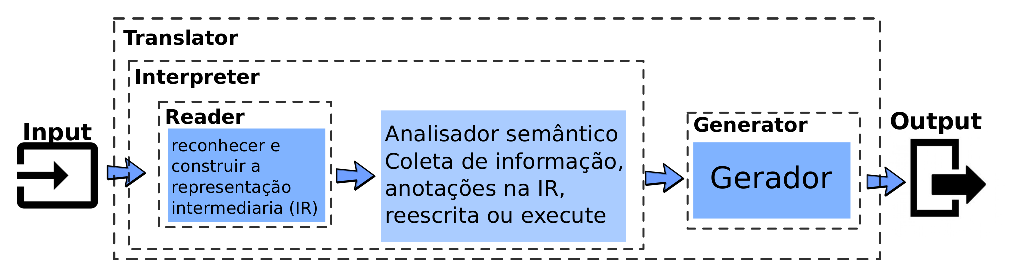
\includegraphics[scale=0.9]{Imagens/stagesLanguageApp}
	\label{fig:stagesLanguageApp}
	\caption{Fases de aplicações com linguagens.}
\end{figure}

Aplicações de manipulação de linguagem de programação é um trabalho desafiador e complicado por isso é necessário dividir este trabalho em componentes que quando combinados proporcionam a análise e manipulação de uma linguagem. Com isso é permitido que uma entrada válida seja trabalhada e convertida para que esta se torne uma saída que internamente é uma entrada interna de um outro estágio deste processo confome exemplificado na Figura:~\ref{fig:stagesLanguageApp}. 

Atualmente existe um esforço para tratar a engenharia de linguagens de programação como sendo o desenvolvimento de um software comum. Algumas aplicações típicas deste domínio são \texttt{reconhecedor, interpretador, tradutor, generator} conforme menciona Terrance Parr em~\cite{Parr:2009:LIP:1823613},  além de \texttt{ferramentas para a identificação de bugs}. Uma dessas é a ferramenta \textit{FindBugs}~\cite{FindBugs} a qual faz uso de alguns dos estágios descritos por Terance Parr em ~\cite{Parr:2009:LIP:1823613}.

A combinação de algumas das ferramentas citadas anteriormente, originou o \textit{FindBugs}~\cite{FindBugs} que é uma ferramenta desenvolvida em Java que processa o \texttt{bytecode} para identificar padões de erros. A Figura:~\ref{fig:findBugs} demonstra no mais alto nível a junção de algumas ferramentas. 

\begin{figure}[h]
	\center
	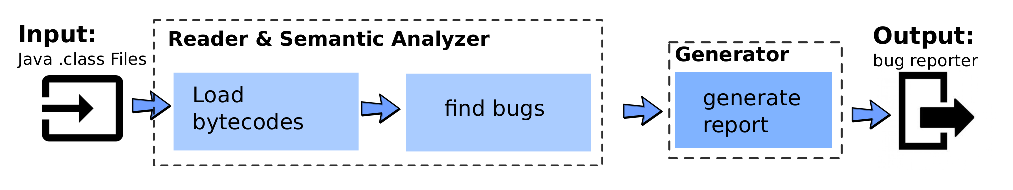
\includegraphics[scale=0.9]{Imagens/pipelineFindbugs}
	\label{fig:findBugs}
	\caption{Fase do pipiline do FindBugs.}
\end{figure}

Especificamente no caso deste trabalho é necessário a contrução de um software que realiza análise estática de código para identificar o uso e oportunidades do uso construções da linguagem Java. E para isso a Figura:~\ref{fig:stagesAnalyzer} exemplifica no alto nível as ferramentas qua compõem o analisador.

\begin{figure}[h]
	\center
	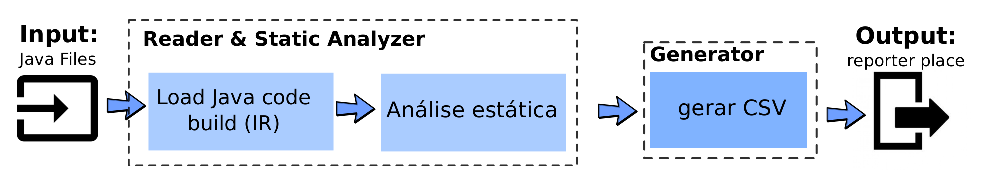
\includegraphics[scale=0.9]{Imagens/stagesAnalizer}
	\label{fig:stagesAnalyzer}
	\caption{Ferramentas necessárias para contrução do analisador estático.}
\end{figure}

%\begin{itemize}
%	\item \textit{Reader:} É uma contrução capaz de receber uma estutura de dado como um input ou um fluxo de inputs. O fluxo de input pode geralmente é texto puro mas pode ser utilizado dado binário. Como exemplo de aplicação tem-se ferramentas analisadoras de referências cruzadas, e ferramantas para carregar classes.
%	
%	\item \textit{Generator:} Percorre uma estutura de dado e emite uma saída. Como exemplo tem-se ferramentas de mapeamento de objetos relacionais em banco de dados, serializador de objetos, gerador de código fonte e geradores de página web.
%	
%	\item \textit{Translator or Rewriter:}A partir um input de texto ou binário é emitido uma saída para uma linguagem que pode ser a mesma ou não. É a combinação do \textit{reader} e \textit{generator}. COmo exemplo tem-se tradutores de linguagens extintas para linguagens atuais, \texttt{refactorers},  gerador de logs e macro pre-processadores.
%	
%	\item \textit{Interpreter:} Um interpretador, lê uma entrada, decodifica e executa as instruções, interpretadores variam de simples calculadoras até a implementação de linguagens de programação como Java, Python e PHP.
%\end{itemize}





Um ponto crítico quanto a análise de código fonte é o \textit{parser} da linguagem, onde é necessário reconhecer uma frase para efetuar a interpretação ou fazer a tradução para que a criação da representação intermediária aconteça. Inicialmente é necessário identificar se a frase que será tratada é um \textit{assignment} ou uma chamada de função.
 
Reconhecer uma frase acarreta em duas coisas, distingui-la de outras construções e identificar os elementos e as subestruturas que compõem esta frase. Por exemplo se uma frase for reconhecida como um \textit{assignment}, pode-se identificar as variáveis a esquerda do operador \texttt{=} e uma expressão que é a subestrutura a direita. Este ato de reconhecer uma frase é denominado \textit{Parse}.

\section{Parse}

Para conceber uma ferramenta de análise de código é necessário gerar um \textit{parse} do código fonte o que torna isto uma tarefa complexa e desafiadora. Entretanto existem alguns padrões e neste será aborda os 4 mais importantes segundo Terence Parr em \cite{Parr:2009:LIP:1823613}.
\begin{itemize}
	\item \textbf{Mapping Grammars to Recursive-Descent Recognizers}\\
	Sua proposta é traduzir uma gramática para uma recursão descendente para reconhecer frases e sentenças em uma linguagem especificada por uma gramática. Este pradrão identifica o núcleo do fluxo de controle para qualquer recursão descendente e é utilizado nos 3 padrões seguintes. 
	Para construir um reconhecedor léxico ou \textit{parsers} manualmente o melhor ponto de início é a gramática, com isso este padrão fornece uma maneira simples de construir reconhecedores diretamente de sua gramática.
	
	\item \textbf{LL(1) Recursive-Descent Lexer}\\
	O objetivo deste pradrão é para emitir uma sequência de símbolos. Cada símbolo tem dois atributos primários: um tipo de \textit{token}(símbolo da categoria) e o texto associado por exemplo 
	no português, temos categorias como verbos e substantivos, bem como símbolos de pontuação, como vírgulas e pontos. Todas as palavras dentro de uma determinada categoria são do mesmo tipo de \textit{token}, embora o texto associado seja diferente. O tipo de nome do \textit{token} representa o categoria identificador. Então precisamos tipos de \textit{token} para o vocabulário \textit{string} fixa símbolos como também lidar com espaços em branco e comentários.
	\item \textbf{LL(1) Recursive-Descent Parser}\\
	Esse é o mais conhecido padrão de análise descendente recursiva. Ele só precisa	a olhar para o símbolo de entrada atual para tomar decisões de análise. Para cada regra de gramática, existe um método de análise no analisador. Este padrão analisa a estrutura sintática da sequência sinal de uma frase usando um único \textit{token} \textit{lookahead}. Este analisador pertence à LL(1) classe do analisador de cima para baixo, em especial, porque usa um único sinal de verificação à frente (daí o "1" no nome). É o principal mecanismo de todos os padrões de análise subsequentes. Este padrão mostra como implementar as decisões de análise que utilizam um símbolo único da visão antecipada. É a forma mais fraca de descendente recursivo parser, mas o mais fácil de compreender e aplicar.
	\item \textbf{LL(k) Recursive-Descent Parser}\\
	Este padrão utiliza a o modo \textit{top-down} para percorrer um árvore semântica com o auxílio de expressões booleanas que ajudam na tomada de decisão e estas expressões são conhecidas como predicados semânticos.
	
\end{itemize}

\section{Análise estática}
Análise estática é uma técnica automática no processo de verificação de software realizado por algumas ferramentas sem a necessidade de que o software tenha sido executado. Para Java exitem duas possibilidades de realizar tal análise na qual uma das técnicas realiza análise no código fonte e a outra a realiza no {\it bytecode} do programa segundo ~\cite{Ayewah:2008:USA:1439186.1439221}. Neste trabalho ser utilizada a pesquisa baseada no código fonte sem que tenha sido executado devido a flexibilidade e infraestrutura consolidada encontrada no eclipse AST.

Um fato importante é que tal análise somente obtém sucesso se forem determinados padrões ou comportamento para que sejam pesquisados no software. Neste projeto o tais comportamentos são determinados por {\it visitors} conforme explica Gamma et. al. ~\cite{Gamma:1995} devido a toda infraestrutura a qual as ferramentas do eclipse fornecem facilidade para que seja realizada uma análise baseada em padrões.

Devido a este trabalho de verificação de software é possível detectar falhas de forma precoce nas fases de  desenvolvimento evitando que bugs e falhas sejam introduzidas e até mesmo postergados e isso é uma vantagem existe a economia de tempo com falhas simples, {\it  feedback} rápido para alertar a equipe devido as falhas ocorridas e pode-se ir além de simples casos de testes podendo aprimorar estes para que  fiquem mais rigorosos pois a partir do momento que o analisador encontrar uma falha é possível criar um teste de caso para que esta seja testada aumentando a confiabilidade do software.

Existe limitações nestes verificadores estáticos como em software desenvolvidos sem qualquer uso de padrões ou sem arquiteturas consolidadas, criado por equipes composta de desenvolvedores inexperientes o qual a ferramente poderá apontar erros que são falsos positivos que são erros detectados que não existem pois o analisador pesquisa por padrões e estruturas consolidadas. Tais problemas são desagradáveis porém não oferecem riscos ao desenvolvimento, podem afetar outras áreas como a de {\it refactoring} a qual poderá encontrar dificuldade em melhorar um código que não segue padrão. Vale ainda ressaltar que a penalidade de encontrar um falso positivo é a perda de tempo em fazer uma inspeção no código para comprovar se é ou não uma falha. Também há a possibilidade de falsos negativos o que cabe ao programador verificar para evitar que tais limitação do analisador não se propague durante o ciclo de desenvolvimento.
%	\section {Análise léxica}
	Ferramentas que operam em código-fonte conforme \cite{Wichmann95industrialperspective} começam por transformar o código em um série de {\it tokens}, descartando recursos sem importância de o texto do programa, tais como espaços em branco ou comentários ao longo do caminho. A criação do fluxo de sinal é chamado de análise lexical. Regras léxicas muitas vezes usam expressões regulares para identificar fichas.
	Observa-se que a maioria dos {\it tokens} são representados inteiramente por seu tipo, mas para ser útil, o {\it tokens} de identificação requer uma peça adicional de informação: o nome do identificador. Para habilitar o relatório de erro útil mais tarde, os {\it tokens} devem transportar pelo menos um outro tipo de informação com eles: a sua posição no texto-fonte (geralmente um número de linha e um número de coluna). Para as mais simples ferramentas de análise estática, o trabalho está quase concluído neste ponto. Se toda a ferramenta tem que fazer é combinar os nomes de funções, o analisador pode ir através do fluxo de {\it tokens} procurando identificadores, combiná-los com uma lista de nomes de funções, e relatar o resultados.
	
	\section{Parser}
	Um analisador de linguagem usa uma gramática livre de contexto (CFG) indicado por \cite{Chess:2007:SPS:1406221} para coincidir com os {\it tokens} correntes. A gramática é composta por um conjunto de produções que descrevem os símbolos (elementos) na língua. No Exemplo é enumerado um conjunto de produções que são capazes de analisar o fluxo de {\it tokens} de amostra.
	
	\begin{lstlisting}
	stmt := if_stmt | assign_stmt
	if_stmt := IF LPAREN expr RPAREN stmt
	expr := lval
	assign_stmt := lval EQUAL expr SEMI
	lval = ID | arr_access
	arr_access := ID arr_index+
	arr_idx := LBRACKET expr RBRACKET
	\end{lstlisting}
	
	O analisador executa uma derivação, combinando o fluxo de sinal contra as regras de produção. Se cada símbolo é ligado a partir da qual o símbolo foi derivado, uma árvore de análise é formada. Na Figura: \ref{fig:TreeParser} mostra uma árvore de análise criada, usando as regras de produção do exemplo anterior. Omiti-se terminais de símbolos que não carregam nomes \textit{(IF, LPAREN, RPAREN, etc.}), para fazer o principais características da árvore de análise mais óbvia.
	
	\begin{figure}[h]
		\center
		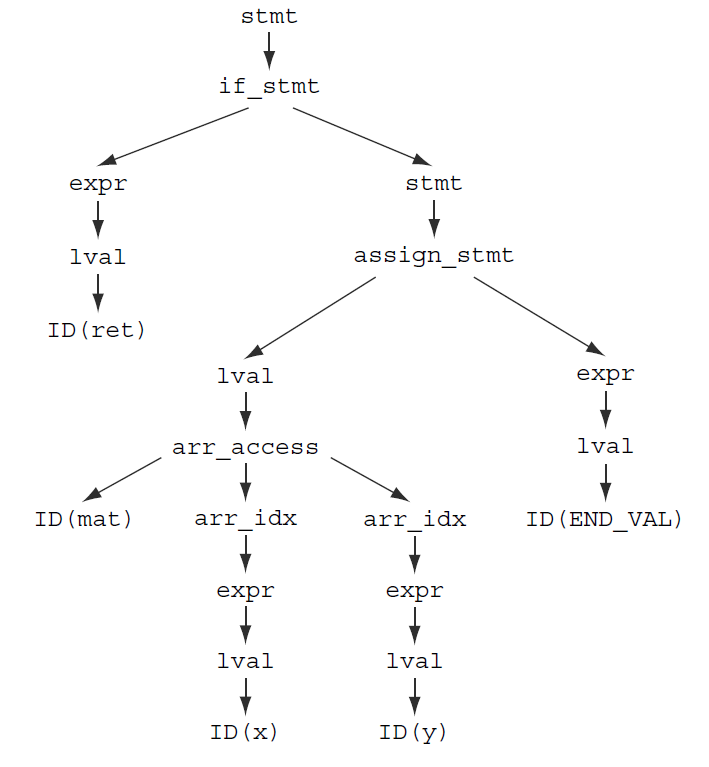
\includegraphics[width=0.8\textwidth]{Imagens/Arvore}
		\label{fig:TreeParser}
		\caption{Árvore de parser.}
	\end{figure}
	
	
	\subsection{Paser JDT Eclipse}
	No caso do \textit{parser} provido pela infraestrutura \textit{JDT} do eclipse,  a classe \textit{ASTParser} contida na biblioteca \textit{org.eclipse.jdt.core.dom} permite a criação de uma árvore de sintaxe abstrata.\\
	Este procedimento é realizado em todos os aquivos \textit{.java} contido em um projeto e com isso cada um possui uma referência de \textit{CompilationUnit} o qual permite acesso ao nó raiz árvore sintática de cada arquivo. O parse é gerado conforme as últimas definições da linguagem utilizando \textit{AST.JLS8}.\

	\begin{lstlisting}
		ASTParser parser = ASTParser.newParser(AST.JLS8);
		
		Map<String, String> options = JavaCore.getOptions();
		options.put(JavaCore.COMPILER_COMPLIANCE, JavaCore.VERSION_1_8);
		options.put(JavaCore.COMPILER_CODEGEN_TARGET_PLATFORM, JavaCore.VERSION_1_8);
		options.put(JavaCore.COMPILER_SOURCE, JavaCore.VERSION_1_8);
		
		parser.setKind(ASTParser.K_COMPILATION_UNIT);
		parser.setCompilerOptions(options);
		parser.setSource(contents);
		
		final CompilationUnit cu = (CompilationUnit) parser.createAST(null);
		return cu;
	\end{lstlisting}
	
	Neste, o \textit{parser} é realizado através de uma classe denominada de mesmo nome, a qual é instanciada um única vez no projeto através do padrão \textit{singleton} \cite{Gamma:1995}.
	

	\section{Sintaxe abstrata}
	É possível fazer uma análise significativa em uma árvore de parser, e certos tipos de checagem estilísticas são mais bem executadas em uma árvore de análise, pois contém mais representações diretas do código assim como o programador escreve. No entanto, executar análise complexa em uma árvore de análise pode ser inconveniente. Os nós da árvore são derivados diretamente das regras de produção da gramática, e essas regras podem-se introduzir símbolos não terminais que existem apenas para fins de fazer a análise mais fácil e menos ambígua, ao invés de para o objetivo de produzir uma facilmente compreendido a árvore. É geralmente melhor para abstrair ambos os detalhes da gramática e as estruturas sintáticas presente no código fonte do programa. Uma estrutura de dados que faz estas coisas é chamado de uma árvore de sintaxe abstrata (AST). O objectivo da AST é fornecer uma versão padronizada do programa adequado para posteriores análises. A AST é normalmente construída associando código construção árvore com regras de produção da gramática. A Figura: \ref{fig:ArvoreAST} mostra uma AST. Observa-se que a instrução {\it if} agora tem uma outra ramificação vazia, o predicado testado pelo caso é agora uma comparação explícita para zero (o comportamento exigido pelo C), e acesso à matriz é uniformemente representada como uma operação de binário.
	
	\begin{figure}[h]
		\center
		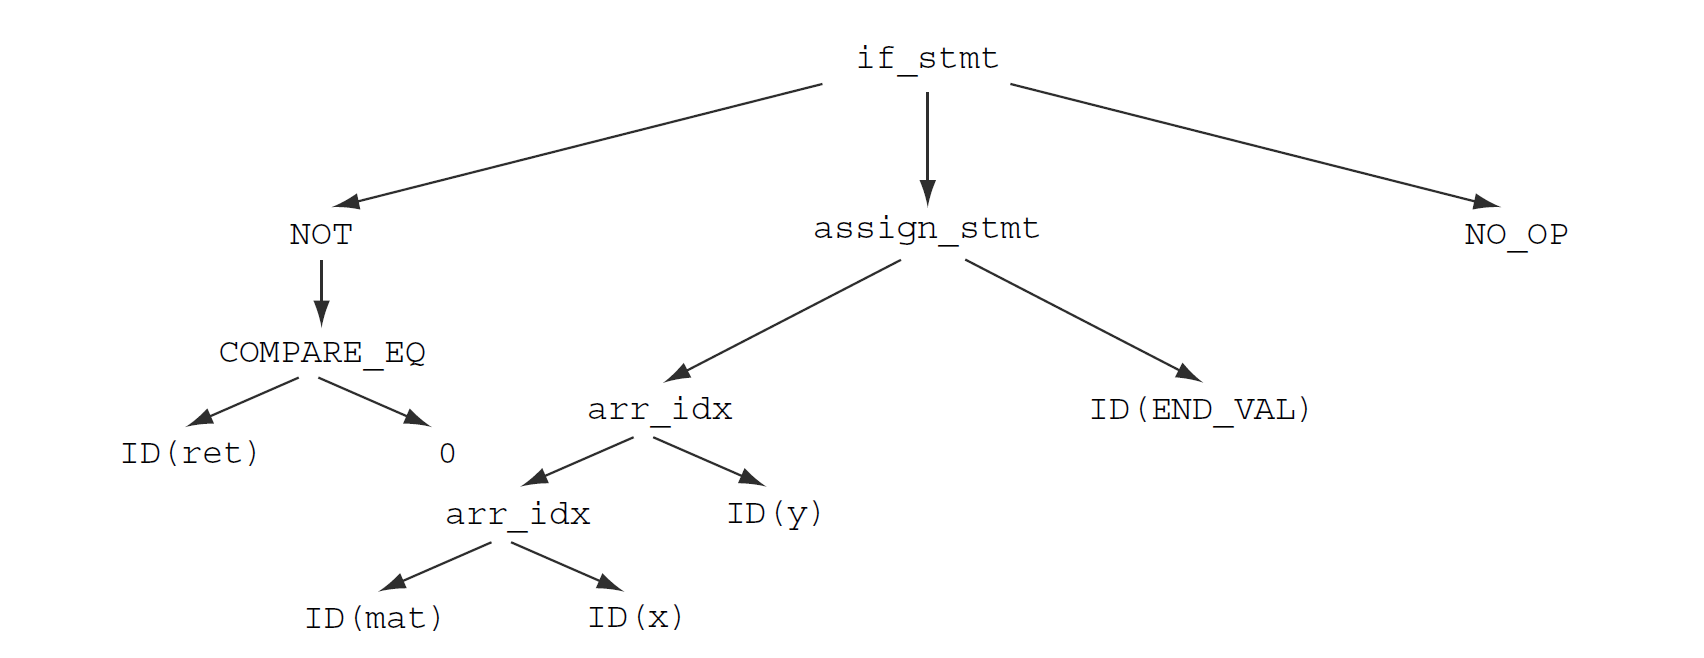
\includegraphics[width=1\textwidth]{Imagens/ArvoreAST}
		\label{fig:ArvoreAST}
		\caption{Árvore AST.}
	\end{figure}

	\section{Análise semântica}
	Como a AST está sendo construída, a ferramenta cria uma tabela de símbolos ao lado dela. Para cada identificador no programa, a tabela de símbolos associa o identificador com seu devido tipo e um ponteiro para a sua declaração ou definição. Com a AST e a tabela de símbolo, a ferramenta está agora equipado-se para realizar a verificação de tipo. A ferramenta de análise estática não pode ser obrigados a comunicar erros de checagem de tipo da maneira um compilador faz, mas informações de tipo é criticamente importante para a análise de uma linguagem orientada a objetos, porque o tipo de um objeto determina o conjunto de métodos que o objeto pode invocar. Além disso, é normalmente desejável para converter, pelo menos, as conversões do tipo implícito no código fonte para conversões de tipo explícitas no AST. Por estas razões, uma ferramenta de análise estática avançado tem a ver apenas como muito trabalho relacionado com a verificação de tipo como um compilador faz. No mundo do compilador, resolução de símbolo e verificação de tipo são referidos como análise semântica porque o compilador está atribuindo significado aos símbolos encontrada no programa. As ferramentas de análise estática que usam essas estruturas de dados têm uma vantagem distinta sobre ferramentas que não o fazem. Por exemplo, eles podem interpretar corretamente o significado dos operadores sobrecarregados em C++ ou determinar que um método em Java chamado doPost () é, na verdade, uma parte de uma implementação de HttpServlet.Estas capacidades permitem uma ferramenta para executar verificações úteis na estrutura deo programa. Após análise semântica, compiladores e a análise estática mais avançada ferramentas de formas de peça. Um compilador moderno usa a AST e o símbolo e o tipo informações para gerar uma representação intermediaria, uma versão genérico do código de máquina que é adequado para otimização e, em seguida, a conversão em específico da plataforma de código-objeto. O caminho para ferramentas de análise estática é menos clara. Dependendo do tipo de análise a ser realizada, uma ferramenta de análise estática pode executar transformações adicionais sobre a AST ou pode gerar a sua própria variedade de representação intermediária adequada às suas necessidades. Se uma ferramenta de análise estática usa sua própria representação intermediária, que, geralmente, permite a atribuição, pelo menos, ramificando, {\it looping}, e chamadas de função. A representação intermediária que uma ferramenta de análise estática usa é geralmente umvista de nível superior do programa do que a representação intermediária que um compilador usa. Por exemplo, um compilador de linguagem C, provavelmente, converter todas as referências a campos para estruturar deslocamentos em {\it byte} na estrutura pela sua representação intermediaria, enquanto uma ferramenta de análise estática mais provavelmente continuará para se referir a estrutura de campos, pelos seus nomes.

  \postextual
  \bibliographystyle{plain}
  \bibliography{referencias/referencias}

\end{document}
